%%%%%%%%%%%%%%%%%%%%%%%%%%%%%%%%%%%%%%%%%%%
\section{Module Action Semantics}
\label{sect:actSemantics}
%%%%%%%%%%%%%%%%%%%%%%%%%%%%%%%%%%%%%%%%%%%

This section provides a formal definition of \textit{module action} that is based on the UML Action language~\cite{omg_unified_2017}. %
%, which is suitable for use with the activity graph language \agl~that we propose in Section~\ref{sect:agl}. 
Our definition focuses on describing the structure of module action and its pre- and post-states. %
%State is an intrinsic part of behavioral specification~\cite{omg_unified_2017}.
%
We recursively define module action by beginning with the most primitive type of action called \textit{atomic action}. We then combine these actions to form \textit{atomic action sequence} and, more generally, \textit{structured atomic action}, resulting in a precise specification of the behavioral semantics of modules in MOSA. 

%\subsection{A Formalism for Module Action} 
%%%%%%%%%%%%%%%%%%%%%%%%%%%%%%%%%%%%%%%%%%%%
\subsection{Atomic Action} \label{sect:arch-atomic-action}
%%%%%%%%%%%%%%%%%%%%%%%%%%%%%%%%%%%%%%%%%%%
Although each module is different, we observe that there exists a set of primitive behaviors that underlie all modules. We capture these primitive behaviors in what we term \textit{atomic actions}.
%
\begin{definition} \label{def:atomic-action}
An \textbf{atomic action} is a smallest meaningful module behavior provided to an actor (which is either a human or another module/system) through the view for manipulating the domain objects of the domain class.
%
Atomic action is characterised by: 
\begin{itemize}
\item \membern{name}: the action name.
%
\item \membern{preStates} (for \membern{localPrecondition}~\cite{omg_unified_2017}): the states at which a current module must be in order for this action to proceed.
%
\item \membern{postStates} (for \membern{localPostcondition}~\cite{omg_unified_2017}): the states at which the action completes its execution on a current module.
%
\item \membern{fieldValSet} (for \membern{input}~\cite{omg_unified_2017}): captures the input of the action. It is a set of pairs $(f,v)$ where $f$ is the name of a domain field of the domain class, and $v$ is the value assigned to this field by the action. 
%
\item \membern{output}: the domain class for object manipulation actions and empty for all other actions.

Although attribute \membern{name} uniquely identifies an action, for ease of exposition, we usually list two other attributes, \membern{postStates} and \membern{fieldValSet}, with \membern{name}.
%
Thus, we denote by $ a = (o,s,i) $ an atomic action $a$ whose \membern{name}, \membern{postStates}, and \membern{fieldValSet} are $ o $, $ s $, and $i$ (\resp). We use the dot notation to refer to the components, \eg, $ a.\membern{postStates} = s$.\qed
\end{itemize}
\end{definition}

%Note the following about the above definition. 
%First, we use module states to abstract from the local pre- and post-conditions of each action. This abstraction enables us to flexibly combine actions based on states to construct more complex ones. A \textbf{module state} abstracts from the states of the model, view and controller components of a module as these components handle a module action. Certain module states can occur concurrently, resulting in what we call \textbf{concurrent state}s. We write these states using the operator `+'. 
%The \membern{postStates} of primitive action consists of a single state, while that of more complex actions (discussed in Section~\ref{sect:arch-saa}) consists of multiple states.
The above definition has the following points to note. Firstly, module states are used to abstract from the local pre- and post-conditions of each action, which allows for the flexible combination of actions based on states to construct more complex ones. A module state represents the states of the model, view, and controller components of a module as these components handle a module action. Certain module states can occur concurrently, which we refer to as concurrent states and are represented using the `+' operator. The \membern{postStates} of a primitive action consist of a single state, while that of more complex actions (which will be discussed in Section~\ref{sect:arch-saa}) consists of multiple states.

%Second, because each action concerns manipulating the values of some domain fields of the domain class, the action inputs, if any, need to be those that are used for updating these fields. Thus, we define action inputs as a (possibly empty) field-value set. An element of this set is a pair $(f,v)$, where $f$ is a field name and $v$ is a value. The value $v$ in each pair is either specified by the user or from another action that has previously been performed. The latter case occurs when we compose actions together to form more complex behavior. We will explain action composition in the subsequent subsections.
%%We look up the fields using field names and use  their data types as types of the input parameters of the action.
Secondly, another important aspect of the actions is the input values they require. Since actions manipulate domain fields, their inputs need to correspond to the fields they modify. Thus, we define action inputs as a set of field-value pairs, which can be empty. The value in each pair can either be provided by the user or come from a previous action in a composed behavior. In the following subsections, we will discuss how actions can be combined to form more complex behavior.

%Third, the action output consists of at most one type, which is the domain class of the current module. Further, only the object manipulation actions have this output; other actions have an empty output because they do not produce any real output value.
Thirdly, the action output consists of, at most, one type, which corresponds to the domain class of the current module. It's worth noting that only the object manipulation actions have this output; other actions have an empty output because they do not produce any real output value.

%\vspace{-0.4cm}
\begin{table}[ht]
	\setlength\tabcolsep{1pt}
	\centering
	\footnotesize
	\caption{The core atomic actions}\label{tab:core-atomic-actions}
	\begin{tabular}{|>{\centering\arraybackslash}m{2.7cm}|>{\centering\arraybackslash}m{5.6cm}|>{\centering\arraybackslash}m{1.9cm}|>{\raggedright\arraybackslash}m{4.8cm}|}
		%content
		\hline
		\rowcolor{lightgray}
		\textbf{Name} & \textbf{Pre-states}  & \textbf{Post-states} & \textbf{Description} \\\hline
		\membern{open} & \{\code{Init}\} & \{\code{Opened}\} & Open the module's view presenting the domain class. \\\hline
		\membern{newObject} & \{\code{Opened}, \code{Created}, \code{Updated}, \code{Reset}, \code{Cancelled}\} & \{\code{NewObject}\} & Remove from the view any object currently presented and prepare the view for creating a new object. \\\hline
		\membern{setDataFieldValues} & \{\code{NewObject}, \code{Editing}, \code{Created}, \code{Updated}, \code{Reset}, \code{Cancelled}\} & \{\code{Editing}\} & Set values for a sub-set of the view's data fields. \\\hline
		\membern{createObject} & \{\code{NewObject}, \code{Editing} + \code{ObjIsNotPresent}\} & \{\code{Created}\} & Create a new object from data entered on the view. The created object is presented on the view.\\\hline
		\membern{updateObject} & \{\code{Editing} + \code{ObjIsPresent}\} & \{\code{Updated}\}& Update the current object from data entered on the view. The updated object remains on the view.\\\hline
		\membern{deleteObject} & \{\code{Created}, \code{Updated}, \linebreak \code{Reset} + \code{ObjIsPresent}, \linebreak \code{Cancelled} + \code{ObjIsPresent}\} & \{\code{Deleted}\} & Delete the current object. The deleted object is removed from the view.\\\hline
		\membern{reset} & \{\code{Editing}\} & \{\code{Reset}\} & Initialise the view to redisplay the current object (discarding all user input).\\\hline
		\membern{cancel} & \{\code{NewObject}, \code{Editing} + \code{ObjIsNotPresent}\} & \{\code{Cancelled}\} & Cancel creating a new object (discarding all user input, if any).\\\hline
	\end{tabular}
\end{table}

Table~\ref{tab:core-atomic-actions} lists definitions of the core atomic actions. %
For exposition purposes, we divide the actions into two groups. %
The first group includes actions that concern the overall operational context of the module.
The actions in this group include \membern{open}, \membern{newObject}, \membern{setDataFieldValues}, \membern{reset}, and \membern{cancel}. The post-states of these actions consist of the following states: \code{Opened}, \code{NewObject}, \code{Editing}, \code{Reset}, and \code{Cancelled} (\resp). 
%
The second group includes three essential domain object manipulation actions: \membern{createObject}, \membern{updateObject}, and \membern{deleteObject}. The post-states of these actions include the following states: \code{Created}, \code{Updated}, and \code{Deleted} (\resp).
%
%We will illustrate the atomic actions in various examples that will be presented later in this paper.

Note from Table~\ref{tab:core-atomic-actions} that only action \membern{setDataFieldValues} requires the \membern{fieldValSet} to be specified as input. Other actions do not require any input and thus, for them, this set is empty. Note also how the two module states \code{ObjIsPresent} and \code{ObjIsNotPresent} can each occur concurrently with any one of the following states: \code{Editing}, \code{Reset}, and \code{Cancelled}. For example, the concurrent state \code{Editing} + \code{ObjIsPresent} means that the module is currently presenting an object on the view and that this object is being edited by the user. In contrast, \code{Editing} + \code{ObjIsNotPresent} means that the module is currently prompting the user to enter input data for a new object. This object has not yet been created.

%%%%%%%%%%%%%%%%%%%%%%%%%%%%%%%%%%%%%%%%%%%%%%%%
\subsection{Atomic Action Sequence (ASE)} \label{sect:arch-ase}
%%%%%%%%%%%%%%%%%%%%%%%%%%%%%%%%%%%%%%%%%%%%%%%%

%In practice, the core atomic actions are combined in sequence to form more useful behavior. This behavior, which we call \textit{atomic action sequence}, corresponds with an interaction scenario. We model this sequence using structured action of UML Activity diagram~\cite{omg_unified_2017}. %
%%
%We denote by $\func{first}$ and $\func{last}$ two functions that return the first and last elements (\resp) in a sequence.
In practice, the core atomic actions are combined in sequence to form more useful behavior. This behavior, which we call \textit{atomic action sequence}, corresponds to an interaction scenario. We model this sequence using structured actions of the UML Activity diagram~\cite{omg_unified_2017}. We denote by $\func{first}$ and $\func{last}$ two functions that return the first and last elements (\resp) in a sequence.

\begin{definition} \label{def:ase}
An \abbrv{atomic action sequence}{ASE} $S = (a_1,\dots,a_n)$ is a module action iff $a_i.\membern{postStates} \subseteq a_{i+1}.\membern{preStates} ~(\forall a_i, a_{i+1} \in S)$. %
%
$S$ has the following properties:
\begin{itemize}
\item $S.\membern{preStates} = \func{first}(S).\membern{preStates}$
\item $S.\membern{postStates} = \func{last}(S).\membern{postStates}$ 
\item $S.\membern{fieldValSet} = \func{first}(S).\membern{fieldValSet}$
\item $S.\membern{output} = \func{last}(S).\membern{output}$ \qed
\end{itemize}
\end{definition}

{\makeatletter
	\let\par\@@par
	\par\parshape0
	\everypar{}
\begin{wrapfigure}{r}{7.1cm}
%\begin{figure}[ht]
	\centering
	\vspace{-2.5cm}
	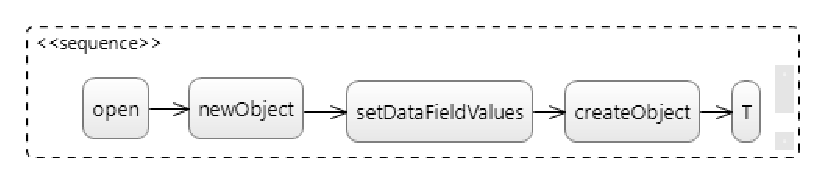
\includegraphics[scale=0.33]{ase-example}
\vspace{-0.1cm}
	\caption{An ASE to create a domain object of type $T$.} %
\vspace{-0.3cm}
	\label{fig:ase-example}
\end{wrapfigure}

\noindent\textbf{Example.} 
%Figure~\ref{fig:ase-example} shows an ASE that creates a new domain object whose type is the domain class $T$ of a module. This ASE consists in a sequence of four atomic actions and is characterised by:\\ \membern{name}=\strq{Sequence:~create~objects},\\
%\membern{fieldValSet}=\attrib{setDataFieldValues}{fieldValSet}=$\emptyset$,\\
%\membern{postStates}=\{\code{Created}\}.\\
%%
%The first atomic action is \membern{open}, which opens the view presenting the domain class. Once completed, this action raises an event with the state \code{Opened}, so that interested listeners of this event can handle. This action then leads to the execution of the second atomic action: \membern{newObject}. This sequence is valid because, as listed in Table~\ref{tab:core-atomic-actions}, \attrib{open}{postStates} $\subset$ \attrib{newObject}{preStates}. Action \membern{newObject} prepares the view so that it is ready to receive input from the user for creating a new object. Once completed, this action raises an event with state \code{NewObject}.
%%
%Because this state is contained in \attrib{setDataFieldValues}{preStates}, we place \membern{setDataFieldValues} as the third action of the ASE. This action is responsible for setting the values of all the view fields, which render the domain fields of the domain class. We place \membern{createObject} as the next (and final) action of the ASE since \attrib{setDataFieldValues}{postStates} $\subset$ \attrib{createObject}{preStates}. This action creates a new domain object with values of the view fields.
Figure~\ref{fig:ase-example} shows an ASE that creates a new domain object of type $T$ in a module. This ASE consists of a sequence of four atomic actions and is characterized by: %
\membern{name}=\strq{Sequence:~create~objects},\\
\membern{fieldValSet}=\attrib{setDataFieldValues}{fieldValSet}=$\emptyset$,\\
\membern{postStates}=\{\code{Created}\}.\\
%
The first atomic action is \membern{open}, which opens the view presenting the domain class. Once completed, this action raises an event with the state \code{Opened}, allowing interested listeners of this event to handle it. This action then leads to the execution of the second atomic action:% 
\par}
\noindent \membern{newObject}. This sequence is valid because, as listed in Table~\ref{tab:core-atomic-actions}, \attrib{open}{postStates} $\subset$ \attrib{newObject}{preStates}. 
%
The \membern{newObject} action prepares the view so that it is ready to receive input from the user for creating a new object. Once completed, this action raises an event with state \code{NewObject}. Because this state is contained in \attrib{setDataFieldValues}{preStates}, we place \membern{setDataFieldValues} as the third action of the ASE. This action is responsible for setting the values of all the view fields, which render the domain fields of the domain class. 
%
We place \membern{createObject} as the next (and final) action of the ASE since \attrib{setDataFieldValues}{postStates} $\subset$ \attrib{createObject}{preStates}. This action creates a new domain object with the values of the view fields.

%A useful property that emerges from our notion of ASE is that there exists a natural multi-level nesting of ASE-backed behaviors along a path in the module containment tree. More specifically, an ASE $S$ is `nested' inside another ASE $S'$ if there exists an activity edge that connects a member action of $S'$ to the start action of $S$. In MOSA, $S'$ is performed on the view of a composite module, and $S$ is on the view of one of its child modules.
%%
%For example, the ASE of \clazz{ModuleStudent} (shown in Figure~\ref{fig:ase-example}) has a nested ASE which is performed on the child module of type \clazz{ModuleEnrolment}. The ASE of \clazz{ModuleStudent} itself is nested inside that of \clazz{ModuleSClass}, thereby creating a 2-level nesting.
%%
%%%%%%%%%%%%%%%%%%%%%%%%%%%%%%%%%%%%%%%%%%%%%%%%%
%%\subsection{Reachable States} \label{sect:arch-reachable-states}
%%%%%%%%%%%%%%%%%%%%%%%%%%%%%%%%%%%%%%%%%%%%%%%%%
%The definition of ASE gives rise to the notion of \textit{reachable state}, which is a module state that is reachable from a given action. We discuss this notion below and use it in the subsequent subsection to define a more generic action composition.

A useful property that arises from our concept of ASE is the natural multi-level nesting of ASE-backed behaviors along a path in the module containment tree. Specifically, an ASE $S$ is considered `nested' inside another ASE $S'$ if there exists an activity edge that connects a member action of $S'$ to the start action of $S$. In MOSA, $S'$ is performed on the view of a composite module, and $S$ is on the view of one of its child modules. 
%
For example, the ASE of \clazz{ModuleStudent} (shown in Figure~\ref{fig:ase-example}) has a nested ASE that is performed on the child module of type \clazz{ModuleEnrolment}. The ASE of \clazz{ModuleStudent} itself is nested inside that of \clazz{ModuleSClass}, thus creating a 2-level nesting. The definition of ASE gives rise to the notion of \textit{reachable state}, which is a module state that can be reached from a given action. We discuss this concept below and use it in the subsequent subsection to define a more generic action composition.

\begin{definition} \label{def:reachable-state}
A module state $s'$ is \textbf{reachable} from an atomic action $a$ if there exists at least one ASE whose first member action is $a$ and whose post-state is $s'$. Action $a$ is called the \textbf{source action} of $s'$. \qed
\end{definition}

%
%\begin{table}[ht]
%	\setlength\tabcolsep{1pt}
%	\centering
%%	\footnotesize
%	\caption{The core atomic actions and their reachable states}\label{tab:reachable-states}
%	\begin{tabular}{|>{\centering\arraybackslash}m{4cm}|>{\arraybackslash}m{12cm}|}
%		%content
%		\hline
%		\rowcolor{lightgray}
%		\textbf{Actions} & \textbf{Reachable states} \\\hline
%		\membern{open} & \code{Opened}, \code{NewObject}, \code{Editing}, \code{Created}, \code{Updated}, \code{Deleted}, \code{Reset}, \code{Cancelled}\\\hline
%		\membern{newObject} & \code{NewObject}, \code{Editing}, \code{Created}, \code{Reset}, \code{Cancelled}\\\hline
%		\membern{setDataFieldValues} & \code{Editing}, \code{Created}, \code{Updated}, \code{Reset} \\\hline
%		\membern{createObject} & \code{Created} \\\hline
%		\membern{updateObject} & \code{Updated} \\\hline
%		\membern{deleteObject} & \code{Deleted} \\\hline
%		\membern{reset} & \code{Reset} \\\hline
%		\membern{cancel} & \code{Cancelled} \\\hline
%	\end{tabular}
%\end{table}

%Clearly, the post-state of an atomic action is reachable from its own action. Table~\ref{tab:reachable-states} lists the reachable states of every atomic action defined in Table~\ref{tab:core-atomic-actions}.
%The first row shows how action \membern{open} can reach all other states. This is because once the module's view is opened, it is ready to perform any of the core atomic actions (in some sequences).
%The rest of the core actions cannot reach state \code{Opened}, because this state is raised only once.
%The second row shows how action \membern{newObject} additionally cannot reach \code{Updated} and \code{Deleted}. This is because this action is reserved for creating a new object. It thus cannot also lead to updating or deleting an existing object.
%The third row shows how action \membern{setDataFieldValues} cannot reach \code{NewObject}, \code{Deleted} and \code{Cancelled}. This is because this action concerns only with inputting data and thus cannot initiate or cancel object creation, nor can it lead to object deletion.
%%
%The last five rows of the table show that the corresponding five actions each has only one reachable state, which are their own states. These actions are ``stubs'', in the sense that they terminate all the ASEs that lead to them.

%Clearly, the post-state of an atomic action is reachable from its own action. Let us define the reachable states of atomic actions shown in Table~\ref{tab:core-atomic-actions}. First, the reachable states of action \membern{open} include \code{Opened}, \code{NewObject}, \code{Editing}, \code{Created}, \code{Updated}, \code{Deleted}, \code{Reset}, and \code{Cancelled}. This is because once the module's view is opened, it is ready to perform any of the core atomic actions (in some sequences). The rest of the core actions cannot reach the state \code{Opened}, because this state is raised only once. Second, the reachable states of \membern{newObject} include \code{NewObject}, \code{Editing}, \code{Created}, \code{Reset}, and \code{Cancelled}. The action 
%\membern{newObject} additionally cannot reach \code{Updated} and \code{Deleted}. This is because this action is reserved for creating a new object. It thus cannot also lead to updating or deleting an existing object.
%Third, the reachable states of action \membern{setDataFieldValues} include \code{Editing}, \code{Created}, \code{Updated}, and \code{Reset}. The action \membern{setDataFieldValues} cannot reach \code{NewObject}, \code{Deleted} and \code{Cancelled}. This is because this action concerns only input data and thus cannot initiate or cancel object creation, nor can it lead to object deletion.
%%
%Finally, with the remaining five actions each has only one reachable state, which is their own states. These actions are ``stubs'', in the sense that they terminate all the ASEs that lead to them.
Clearly, an atomic action can always reach its own post-state. Let us define the reachable states for the atomic actions shown in Table 1. First, the reachable states of the action \membern{open} include \code{Opened}, \code{NewObject}, \code{Editing}, \code{Created}, \code{Updated}, \code{Deleted}, \code{Reset}, and \code{Cancelled}. This is because once the module's view is opened, it is ready to perform any of the core atomic actions (in some sequences). The rest of the core actions cannot reach the state \code{Opened} because this state is only raised once. Second, the reachable states of \membern{newObject} include \code{NewObject}, \code{Editing}, \code{Created}, \code{Reset}, and \code{Cancelled}. Additionally, \membern{newObject} cannot reach \code{Updated} and \code{Deleted} because this action is reserved for creating a new object and cannot lead to updating or deleting an existing object. Third, the reachable states of \membern{setDataFieldValues} include \code{Editing}, \code{Created}, \code{Updated}, and \code{Reset}. This action cannot reach \code{NewObject}, \code{Deleted} and \code{Cancelled} because it concerns only input data and cannot initiate or cancel object creation, nor can it lead to object deletion. Finally, the remaining five actions each have only one reachable state, which is their own state. These actions are ``stubs,'' in the sense that they terminate all the ASEs that lead to them.

\noindent\textbf{Example}. The ASE in Figure~\ref{fig:ase-example} shows that state \code{Created} is reachable from any of the three member actions that precede the action \membern{createObject}. These include \membern{open}, \membern{newObject} and \membern{setDataFieldValues}. 

%%%%%%%%%%%%%%%%%%%%%%%%%%%%%%%%%%%%%%%%%%%%%%%%
\subsection{Structured Atomic Action (SAA)} \label{sect:arch-saa}
%%%%%%%%%%%%%%%%%%%%%%%%%%%%%%%%%%%%%%%%%%%%%%%%

More generally, we observe that a set of related ASEs form a \textit{structured atomic action}. In essence, this action defines a generic behavior that consists of alternative interaction scenarios (each of which is specified by one ASE in the set) that are usually performed (possibly concurrently) by the user.

\begin{definition} \label{def:saa}
	A \abbrv{structured atomic action}{SAA}, \wrt a source atomic action $ a $ and a set of post-states $ E = \{ s_{1},\dots,s_{n} \} $ reachable from $a$, is the set $ A = \{S: ASE ~|~ \func{first}(S) = a, S.\attribn{postStates} \subseteq E \} $, where:
  \begin{itemize}
  \item $A.\membern{preStates}$ = $a.\attribn{preStates}$
  \item $A.\membern{postStates}$ = $E$
  \item $A.\membern{fieldValSet}$ = $a.\attribn{fieldValSet}$
  \item $A.\membern{output}$ = $\bigcup_{S \in A} (S.\attribn{output})$
  \end{itemize}

  Abstractly, we write $ A = (a, \{ s_{1},\dots,s_{n} \}, i) $. If the \membern{fieldValSet} $i$ is $\emptyset$ then we omit it and simply write $A$ as $(a, \{ s_{1},\dots,s_{n} \})$. \qed
  %Abstractly, we write $ A = (a, \{ s_{1},\dots,s_{n} \}) $. \qed
\end{definition}

Clearly, SAA generalizes both atomic action and ASE: An ASE is a single-member SAA, while an atomic action $ a $ is the SAA 
%
%$ (a, \{ a.\membern{postState} \}, a.\membern{fieldValSet}) $. 
$ (a, \{ a.\membern{postState} \}) $.
%
Further, SAA is significantly shorter to compose than an ASE set: All we need to do is specify the start atomic action and the desired post-states.

%\begin{figure}[ht]
%	\centering
%	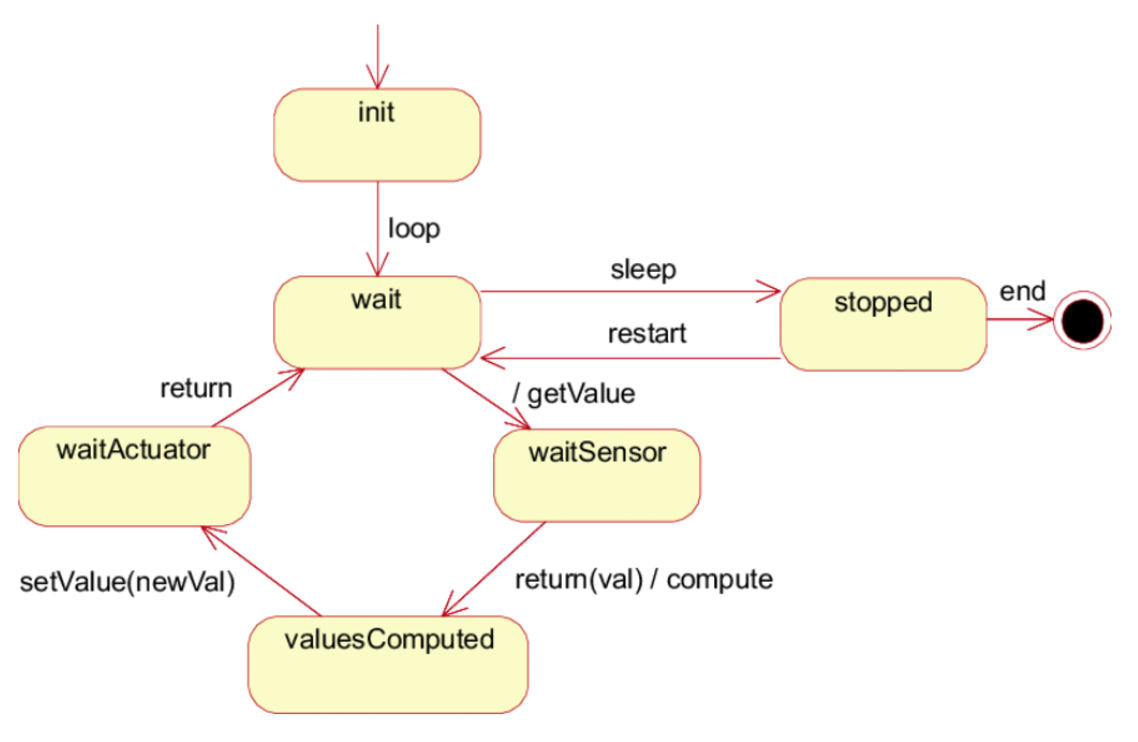
\includegraphics[scale=0.2]{statemachine-example}
%	\caption{Sequences of module action as shown in Table~\ref{tab:core-atomic-actions} could be captured by a state machine.} %
%	\label{fig:statemachine-example}
%\end{figure}
 
\noindent\textbf{Example}. 
%Let us consider the SAA $(\code{newObject}, \{ \code{Created},\code{Cancelled} \})$, which represents a common ASE set that starts with the action \membern{newObject} and ends only when either the state \code{Created} or the state \code{Cancelled} is detected. The ASE set consists of the following frequently-occurring ASEs. The 
%first ASE is the one described earlier in Figure~\ref{fig:ase-example} but excludes the first action. We assume here that the module's view is already opened. The remaining ASEs model alternative scenarios in which the user wants to cancel creating the object at some point between performing the \membern{newObject} action and the \membern{createObject} action.
Let's consider the SAA $(\code{newObject}, \{ \code{Created},\code{Cancelled} \})$, which represents a common set of ASEs that start with the action \membern{newObject} and end only when either the state \code{Created} or \code{Cancelled} is reached. The set consists of frequently-occurring ASEs, such as the one described earlier in Figure~\ref{fig:ase-example}, but excluding the first action. We assume that the module's view is already opened. The remaining ASEs model alternative scenarios in which the user wants to cancel creating the object at some point between performing the \membern{newObject} action and the \membern{createObject} action.


%\subsubsection*{Discussion} %\label{sect:module-act-discussion}

%\noindent {\bf Discussion.} We wish to stress that our definition of module action incorporates the notion of state, which is more formally modeled in another UML behavioral modeling language called Behavior State Machines (BSM) (\S{14.2}~\cite{omg_unified_2017}). The main reason is that the Activity diagram and BSM are tightly linked to states and state transitions to represent behaviors. Indeed, these languages represent two sides of the same coin: the former emphasizes the actual behavior, while the latter focuses on the behavior's effects (states and state transitions). More specifically, a close inspection of the BSM's abstract syntax (\S{14.2.2}~\cite{omg_unified_2017}) reveals that both \clazz{State} and \membern{Transition} have associated \clazz{Behavior}(s) that describe what actually takes place when a particular state is reached or during a transition between some two states. %Figure~\ref{fig:statemachine-example} shows a state machine that could allow us to capture sequences of module actions as shown in Table~\ref{tab:core-atomic-actions}.

%Our notion of module action's pre- and post-states simply looks at the same view but from the behavior's perspective.

%A key difference in our definition of module action, however, is that we allow for a more flexible high-level behavior specification (see Definition~\ref{def:saa}), in which a behavior may terminate at not at most one (as implied in the BSM's specification (\S{14.2.2})) but multiple states. Of course, such a behavior may not terminate freely at any states. In our definition, we precisely specify which reachable states can be used to terminate a module action.

%%%%%%%%%%%%%%%%%%%%%%%%%%%%%%%%%%%%%%%%%%%%%%%%%%%%%%% 
\section{Domain Behavior Patterns}
\label{sect:behaviorPatterns}
%%%%%%%%%%%%%%%%%%%%%%%%%%%%%%%%%%%%%%%%%%%%%%%%%%%%%%%

%This section focuses on explaining our pattern-based approach for incorporating domain behaviors into a domain model. Each domain behavior, that could be captured at a high-level description using a UML activity diagram together with domain-model based statements, is translated into a specification with two parts: (1)~part of the unified class model with new activity classes; and (2)~the activity graph logic of the input activity and the mappings to connect the activity with the unified class model. We realize such a translation by applying a domain behavior pattern. The first catalog of domain behavior patterns is defined as corresponding to the five essential UML activity modeling patterns~\cite{le_domain_2018}, as restrictions to sharpen AGL's semantics domain.
%%as explained in Section~\ref{subsect:domainBehaviors}. 
This section explains our pattern-based approach to incorporating domain behaviors into a domain model. Each domain behavior, described at a high level using a UML Activity diagram and domain-model-based statements, is translated into a specification with two parts: (1)~a part of the unified class model with new activity classes, and (2)~the activity graph logic of the input activity and the mappings to connect the activity with the unified class model. We achieve this translation by applying domain behavior patterns, which are defined as corresponding to the five essential UML activity modeling patterns~\cite{le_domain_2018}, serving as restrictions to sharpen AGL's semantics domain.

%%%%%%%%%%%%%%%%%%%%%%%%%%%%%%%%%%%%%%%%%%%%%%%%%%%%%%% 
\subsection{Specifying Domain Behavior Patterns}
%\label{subsect:specifyBehaviorPatterns}
%%%%%%%%%%%%%%%%%%%%%%%%%%%%%%%%%%%%%%%%%%%%%%%%%%%%%%%

We are particularly interested in the design of the \textit{pattern form}~\cite{riehle_understanding_1996, gamma_design_1994}. To keep the patterns generic, we present for each pattern form a UML Activity diagram and a \textbf{template configured unified class model} that realizes it. The template model is a `parameterized' configured DCSL unified model, in which elements of the non-annotation meta-concepts are named after the generic roles that they play. 
%
For brevity, we omit all associative fields and base domain methods from the model's diagram. 
%
Attached to the template model is an activity graph specification in the \agl~(that is further explained in Section~\ref{sect:agl}). The \agl~specification aims to specify the activity graph logic of the input activity and to maintain the synchronization of current execution states (\wrt the activity) with current states of the domain (\wrt the unified class model).

%We illustrate each pattern of our first catalog with a variant of the DCSL unified model for the enrolment management activity of \courseman. Due to the limitation of the length of this paper, we focus on the \textit{Decisional Pattern} to illustrate the approach. For a detailed explanation of the four remaining patterns, including \textit{Sequential Pattern}, \textit{Forked Pattern}, \textit{Joined Pattern}, and \textit{Merged Pattern}, we refer the reader to our technical report~\cite{dang2023aglTechReport}. 
We provide an example of each pattern in our catalog using a \dcsl unified model for the \courseman enrollment management activity. Due to space constraints, we will only illustrate the \textit{Decisional} pattern in this paper. For more information on the other four patterns (\textit{Sequential}, \textit{Forked}, \textit{Joined}, and \textit{Merged}), please refer to the accompanying technical report~\cite{dang2023aglTechReport}.

%A pattern example includes a configured unified model and one or more software GUIs. In this paper, we will focus on presenting the configured unified model and, in particular, its AGL specification. 

%Please refer to~\cite{le_domain_2018, le_domain_2017} for details about the unified model and the software GUI of each example. The \courseman~software of each example is automatically generated from the configured unified model, using the software tool described in Section~\ref{sect:tool}. 

%%%%%%%%%%%%%%%%%%%%%%%%%%%%%%%%%%%%%%%%%%%%%%%%
%\subsection{Sequential Pattern Form} \label{sect:sequential-pattern}
%%%%%%%%%%%%%%%%%%%%%%%%%%%%%%%%%%%%%%%%%%%%%%%%
%\todo{recapture pattern form image to match other figures}
%
%The top-left of Figure~\ref{fig:sequential-form} shows the UML activity model for \textit{Sequential Pattern}, while the top-right shows the template configured unified model. This model consists of three classes \clazz{Ca}, \clazz{Cs}, and \clazz{Cn}. Class \clazz{Ca} is the activity class and has two associations with the two data classes \clazz{Cs} and \clazz{Cn}. These are the referenced domain classes of the two action nodes $ e_s $ and $ e_n $, \resp
%
%\begin{figure}[ht]
%	\begin{center}
%		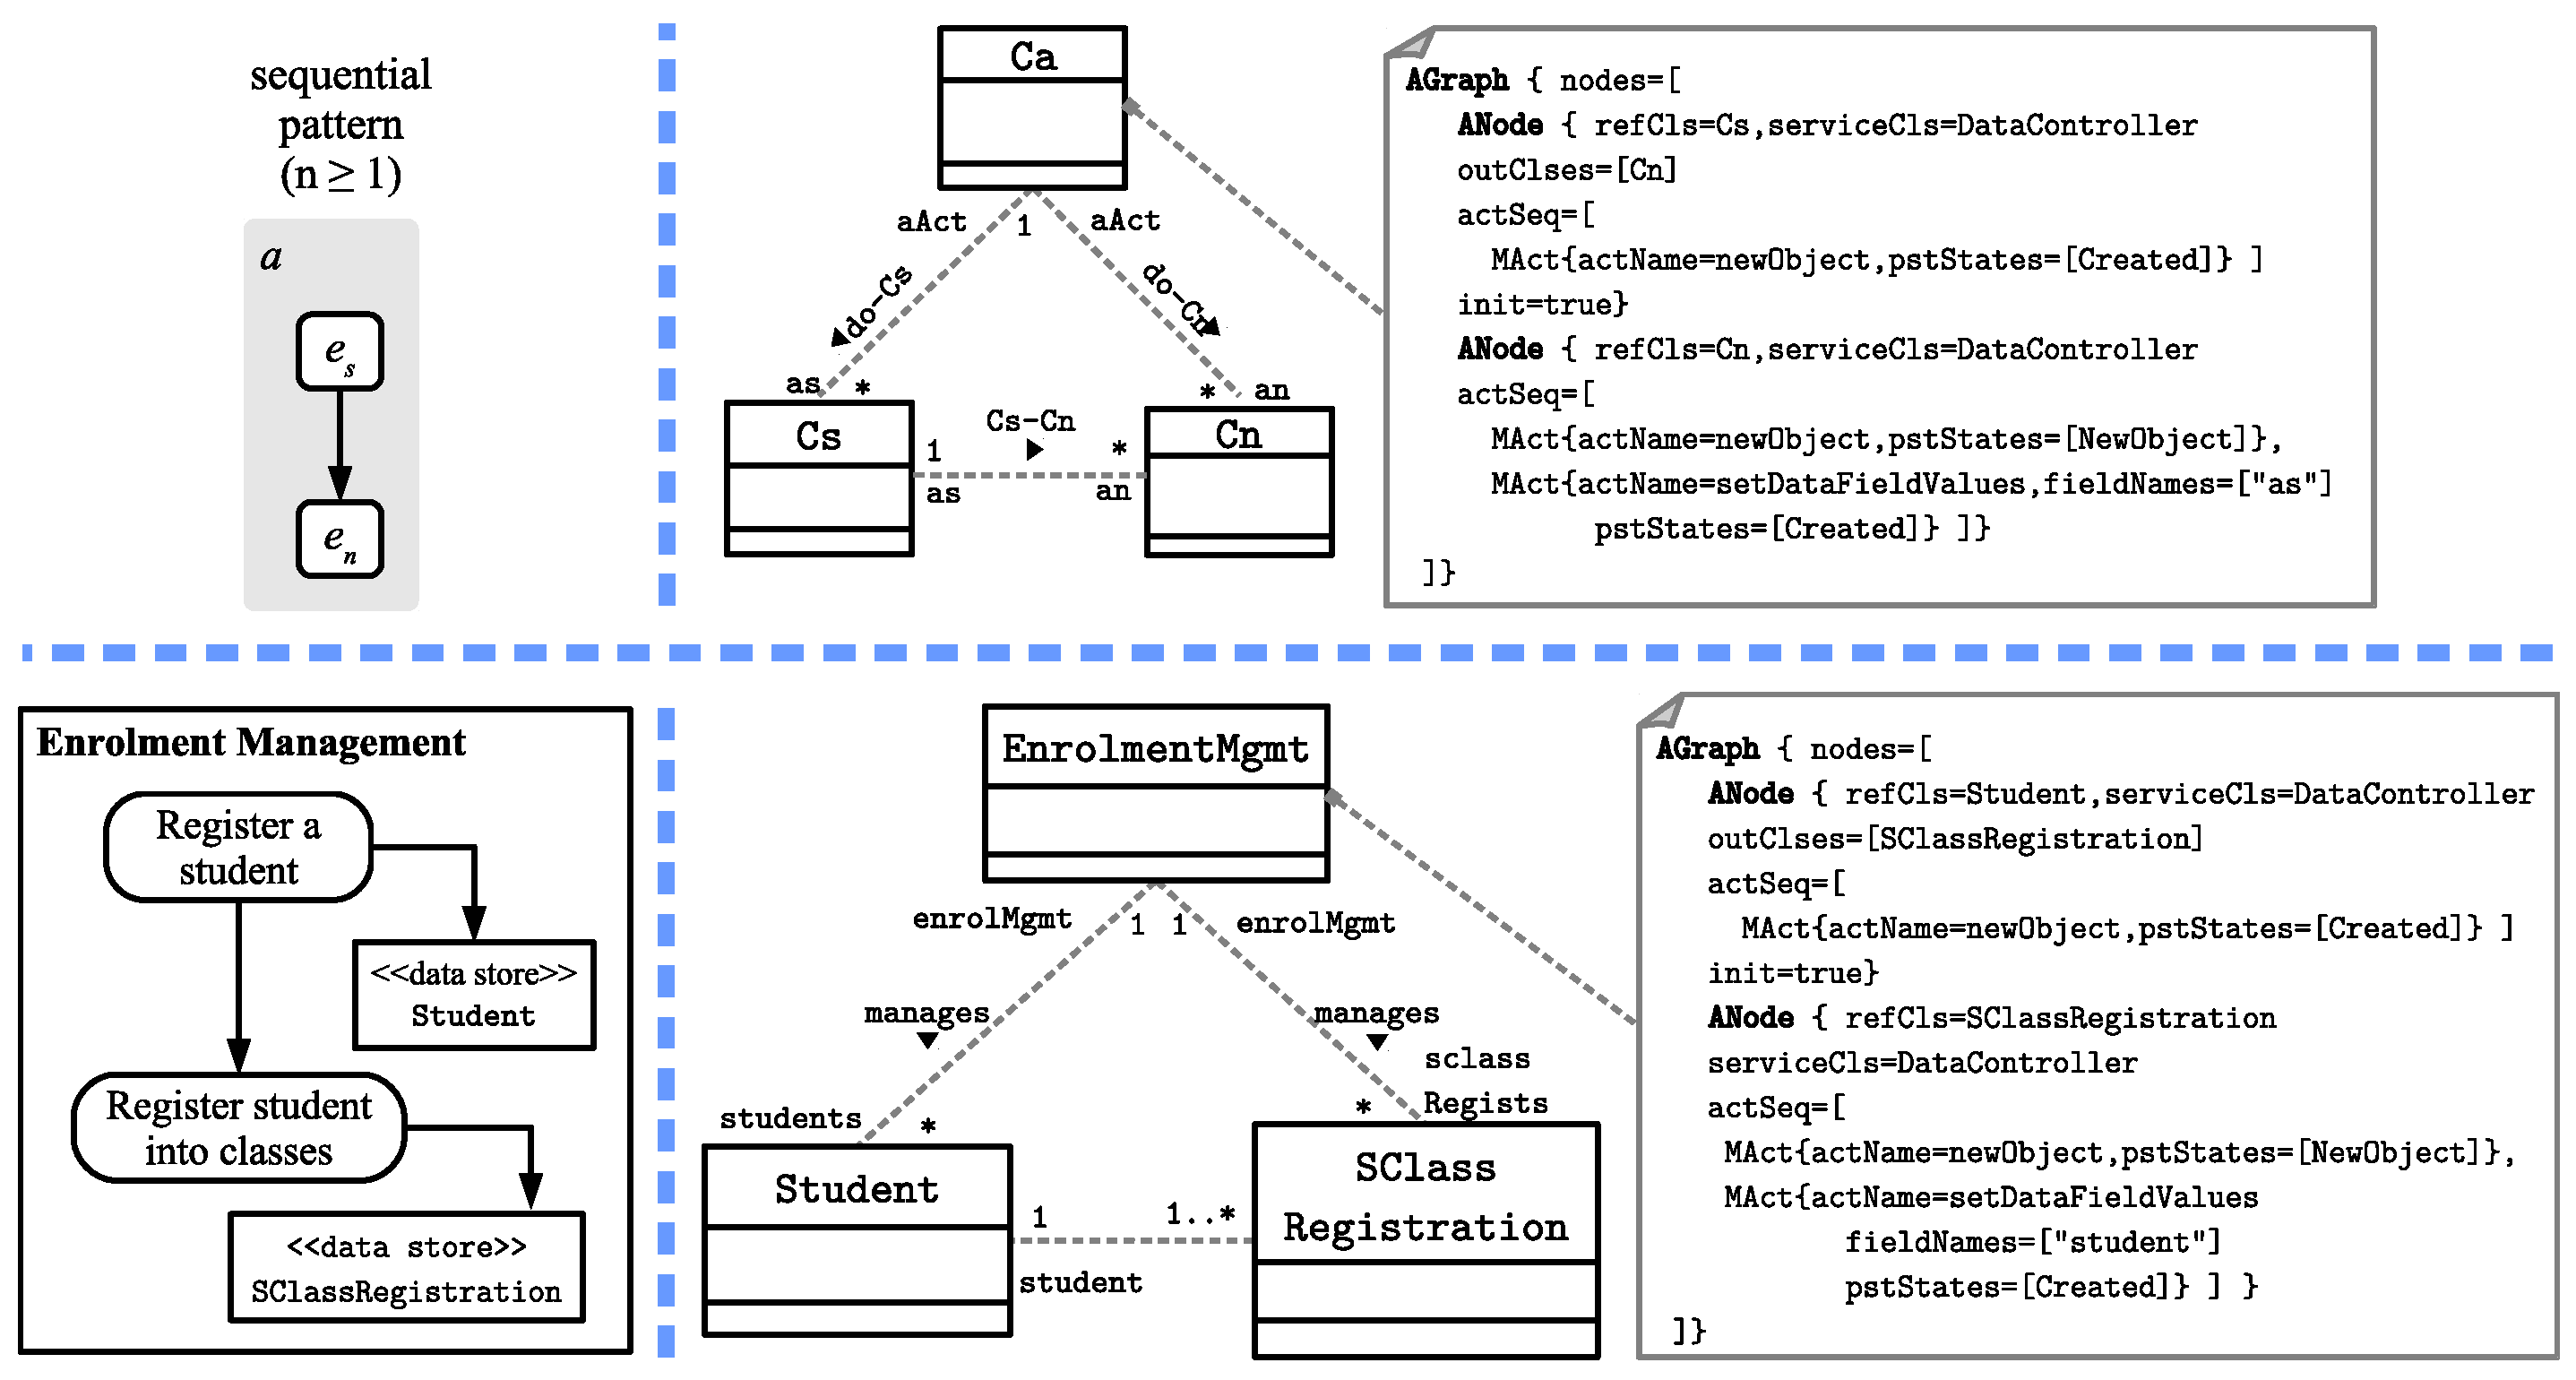
\includegraphics[scale=0.33]{case-study/sequential-form}
%	\caption{The sequential pattern form.} %
%	\label{fig:sequential-form}
%\end{figure}
%
%The AGC is given in the \clazz{AGraph}'s note box in the top-right corner of the figure. It consists of two \clazz{ANode}s. The first \clazz{ANode} specifies node $ e_s $, and the second specifies node $ e_n $. The \clazz{ANode}s are quite self-explanatory except for the three \clazz{MAct}s, which are worth some explanation. The first \clazz{MAct}'s configuration specifies the SAA \amos{newObject}{Created}). %This SAA is a subset of the one presented in Section~\ref{sect:arch-saa}. 
%It involves performing \atomact{newObject}{ NewObject} and any combination of \atomact{setDataFieldValues}{Editing} and \atomact{createObject}{Created}. Action \membern{newObject} is to prepare \clazz{Cs}' view for the user to enter input. Action \membern{setDataFieldValues} is to set a view field's value from each user input (allowing the user to re-enter if an error occurs). And action \membern{createObject} is to create a new \clazz{Cs}' object from the input. 
%
%The second and third \clazz{MAct}s together perform a similar logic over \clazz{Cn}, except for the need to break the \membern{setDataFieldValues} operation into two steps: \textit{(a)} set the \clazz{Cs} object created by the first \clazz{MAct} (and offered by $ e_s $ to $ e_n $ via its output pin) into a suitable view field of \clazz{Cn}'s view and (\textit{b)} set values of other view fields (allowing user to re-enter if an error occurs). To achieve this, the second \clazz{MAct} first specifies \amos{newObject}{NewObject}. The third \clazz{MAct} then specifies the rest of the logic. Step \textit{(a)} is performed by the operation \membern{setDataFieldValues}, which uses the field named \strq{as} to identify the view field of \clazz{Cn}'s view whose value needs to be set. Step \textit{(b)} is performed by \membern{setDataFieldValues} for other view fields.
%
%
%%\subsubsection*{Example}
%\textit{Example}. The bottom of Figure~\ref{fig:sequential-form} shows how the pattern is applied to a simple variant of the \courseman's enrolment management activity. The UML activity model involves performing two actions in sequence. The first action (\clazz{Student}) registers a student into course modules, while the second action (\clazz{SClassRegistration}) registers the student into a preferred class. 
%
%In this example: \clazz{Ca} = \clazz{EnrolmentMgmt}, \clazz{Cs} = \clazz{Student}, $ n $ = 1, \clazz{C1} = \clazz{SClassRegistration}.
%
%\begin{figure}%[ht]
%	\begin{center}
%		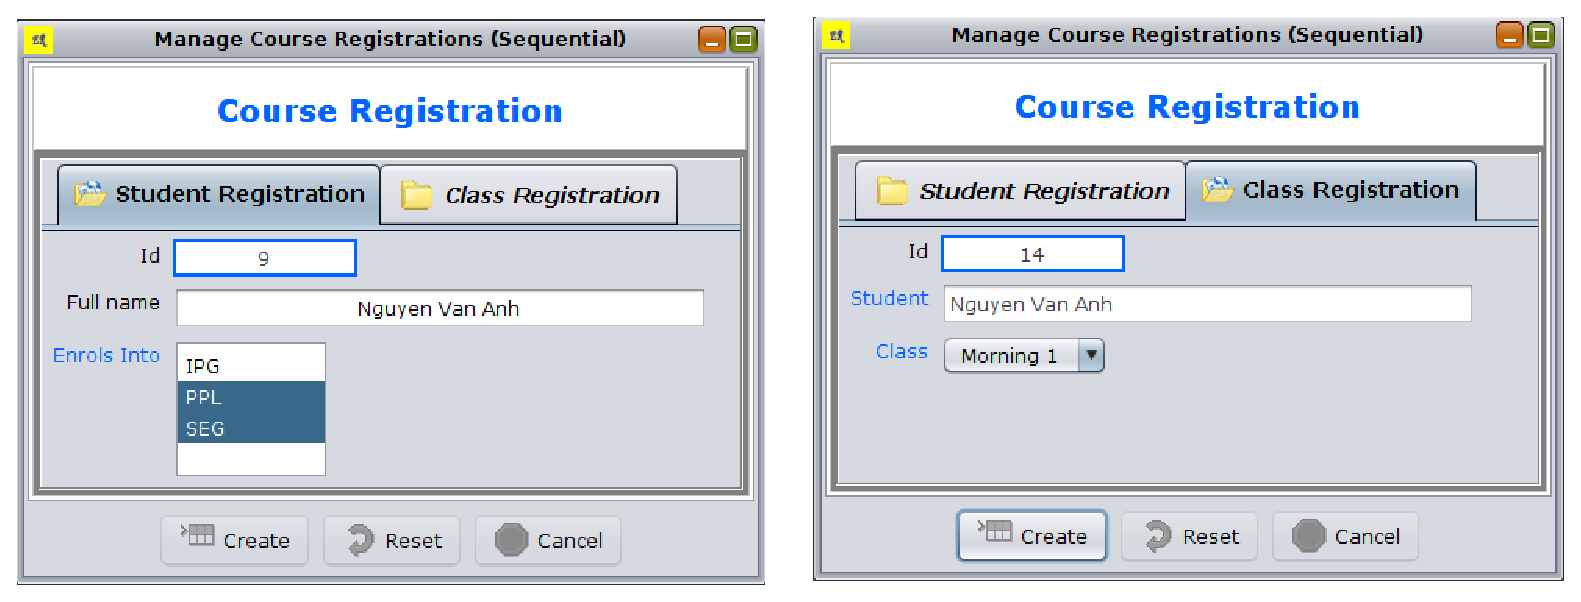
\includegraphics[scale=0.46]{case-study/sequential-form-eg-gui}
%	\end{center}
%	\caption{The sequential pattern form view of enrolment management activity.} %
%	\label{fig:sequential-form-eg-gui}
%\end{figure}
%
%The two GUI snapshots of the example are shown in Figure~\ref{fig:sequential-form-eg-gui}: one snapshot for the view of the one action. Each view is embedded in the \clazz{EnrolmentMgmt}'s view. The overall layout is a tab layout and the view of each associated module is contained in a tab of this layout. The LHS figure shows the tab containing the \clazz{Student}'s view, while the RHS one shows the tab containing the \clazz{SClassRegistration}'s view. Note, in particular, that the view field of the field \clazz{SClassRegistration}.\attribn{student} (i.e., \attrib{Cn}{as} in the template model) is automatically set to the \objc{Student}{\attribn{name}=\strq{Nguyen~Van~Anh}}, which is created on the \clazz{Student}'s view.

%%%%%%%%%%%%%%%%%%%%%%%%%%%%%%%%%%%%%%%%%%%%%%%%
%\subsection{Decisional Pattern Form} \label{sect:decisional-pattern}
%%%%%%%%%%%%%%%%%%%%%%%%%%%%%%%%%%%%%%%%%%%%%%%%%
%The top-left of Figure~\ref{fig:decisional-form} shows the UML activity model, while the top-right shows the template configured unified model. Apart from the activity class \clazz{Ca}, this model includes five other domain classes, namely \clazz{Cd}, \clazz{D}, \clazz{C1}, \clazz{Cn}, and \clazz{Ck}, that are mapped to the five activity nodes. In particular, class \clazz{Ck} is a control class that is referenced by the control node $c_k$ of the activity model. 
%Class \clazz{D} is a decision class, which implements the \clazz{Decision} interface.
%%
%Since the decision's logic may require knowledge of the domain classes involved (namely \clazz{C1}, \clazz{Cn}, and \clazz{Ck}), there are (optional) weak dependency associations between \clazz{D} and these classes. Depending on the domain requirements, we would need none or some of these associations.
The top-left of Figure~\ref{fig:decisional-form} illustrates the UML Activity diagram, while the top-right shows the template configured unified model. Apart from the activity class \clazz{Ca}, this model includes five other domain classes, namely \clazz{Cd}, \clazz{D}, \clazz{C1}, \clazz{Cn}, and \clazz{Ck}, that are mapped to the five activity nodes. In particular, class \clazz{Ck} is a control class referenced by the control node $c_k$ of the activity diagram. Class \clazz{D} is a decision class that implements the \clazz{Decision} interface. Since the decision's logic may require knowledge of the domain classes involved (namely \clazz{C1}, \clazz{Cn}, and \clazz{Ck}), there are optional weak dependency associations between \clazz{D} and these classes. Depending on the domain requirements, we may or may not need some of these associations.

\begin{figure*}[ht]
\begin{center}
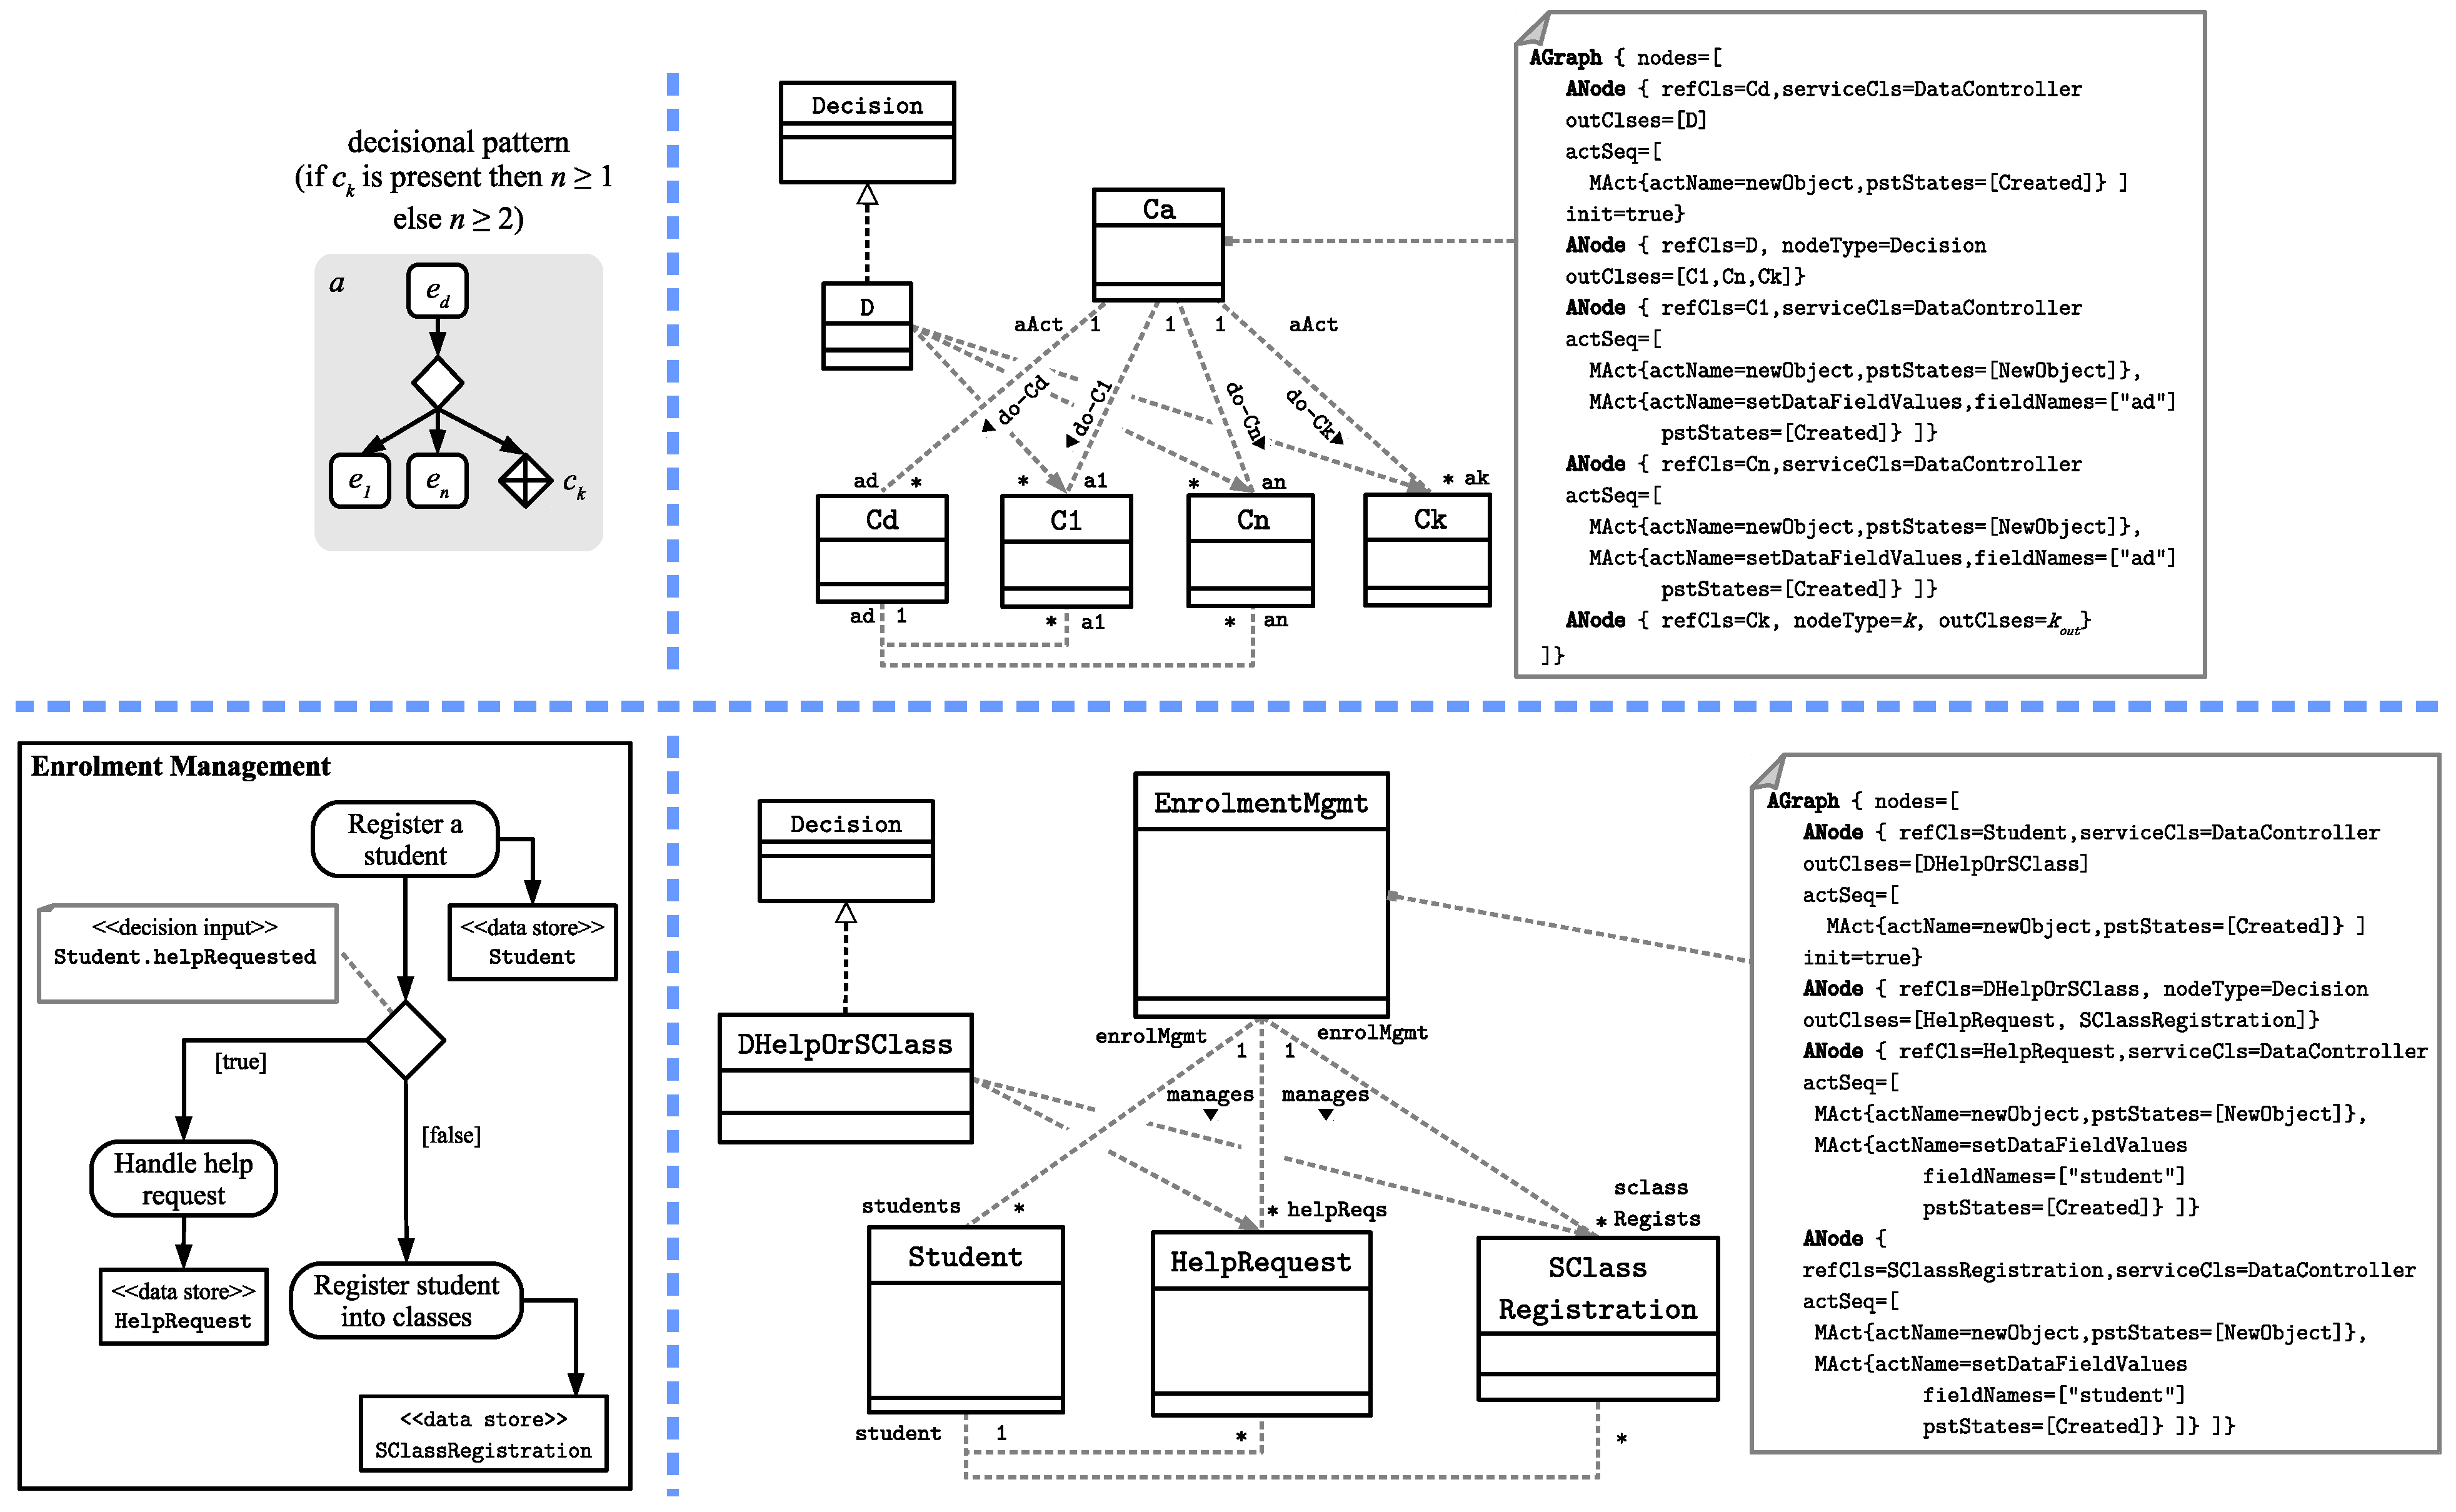
\includegraphics[scale=0.8]{decisional-form}
\end{center}
\vspace{-0.5cm}
\caption{The decisional pattern form.} %
\label{fig:decisional-form}
\vspace{-0.3cm}
\end{figure*}

%Class \clazz{Ca} has one-many associations to the other four domain classes. 
%Note that the association to \clazz{Ck} can be used as a bridge in a larger activity model to other activity flow blocks. This association is applied differently if $ c_k $ is a decision node. In this case, \clazz{Ck} has no associations and thus the association to \clazz{Ck} is replaced by (or ``unfolded'' into) a set of associations that connect \clazz{Ca} directly to the domain classes of the model containing \clazz{Ck}.
%%
%In the template model, the two associations between \clazz{Cd} and \clazz{C1}, \clazz{Cn} reflect the fact that both \clazz{C1} and \clazz{Cn} know about \clazz{Cd}, due to the passing of object tokens from $ e_d $ to $ e_1 $ and $ e_n $ (via the decision node).
The class \clazz{Ca} is associated with the other four domain classes in a one-to-many relationship. It is worth noting that the association with the class \clazz{Ck} can serve as a bridge to other activity flow blocks in a larger activity diagram. However, if $c_k$ is a decision node, \clazz{Ck} has no associations, and the association to \clazz{Ck} is replaced or ``unfolded'' into a set of associations that directly connect \clazz{Ca} to the domain classes of the model containing \clazz{Ck}. In the template model, the two associations between \clazz{Cd} and \clazz{C1}, \clazz{Cn} indicate that both \clazz{C1} and \clazz{Cn} are aware of \clazz{Cd} due to the passing of object tokens from $e_d$ to $e_1$ and $e_n$ via the decision node.

%The AGL specification for this pattern consists of five \clazz{ANode}s. The first \clazz{ANode} is to create a new \clazz{Cd} object. The second \clazz{ANode} is to run the decision logic. The third and fourth \clazz{ANode}s represent the two decision cases: the first results in creating a new \clazz{C1} object for the specified \clazz{Cd} object, and the second, which is repeated for all $ n $, results in creating a new \clazz{Cn} object for the same \clazz{Cd}. The fifth \clazz{ANode} is used for the case that \clazz{Ck} is specified. It uses two variables $ k $ and $ k_{out} $, which are both dependent on \clazz{Ck}. Variable $ k $ specifies the control node type, while variable $ k_{out} $ specifies the array of output domain classes of \clazz{Ck}.
The AGL specification for this pattern includes five \clazz{ANodes}. The first \clazz{ANode} creates a new \clazz{Cd} object, while the second \clazz{ANode} runs the decision logic. The third and fourth \clazz{ANode}s represent the two decision cases: The first creates a new \clazz{C1} object for the specified \clazz{Cd} object, and the second (which is repeated for all $n$) creates a new \clazz{Cn} object for the same \clazz{Cd}. The fifth \clazz{ANode} is used when \clazz{Ck} is specified and involves two variables, $k$ and $k_{out}$, both of which are dependent on \clazz{Ck}. The variable $k$ specifies the control node type, while the variable $k_{out}$ specifies the array of output domain classes of \clazz{Ck}.

\noindent\textbf{Example.} The bottom of Figure~\ref{fig:decisional-form} illustrates how this pattern is applied to \courseman's enrolment management activity. %
%The configured unified model, however, is a more detailed version of the one presented in Figures~\ref{fig:unified-model-example} and~\ref{fig:agc-enrolmentmgmt}. 
In this example, we have: \clazz{Ca} = \clazz{EnrolmentMgmt}, \clazz{Cd} = \clazz{Student}, \clazz{D} = \clazz{DHelpOrSClass}, $ n $ = 2, \clazz{C1} = \clazz{HelpRequest}, \clazz{C2} = \clazz{SClassRegistration}.
The control node $ c_k $ is not specified.

\begin{figure}[ht]
	\begin{center}
		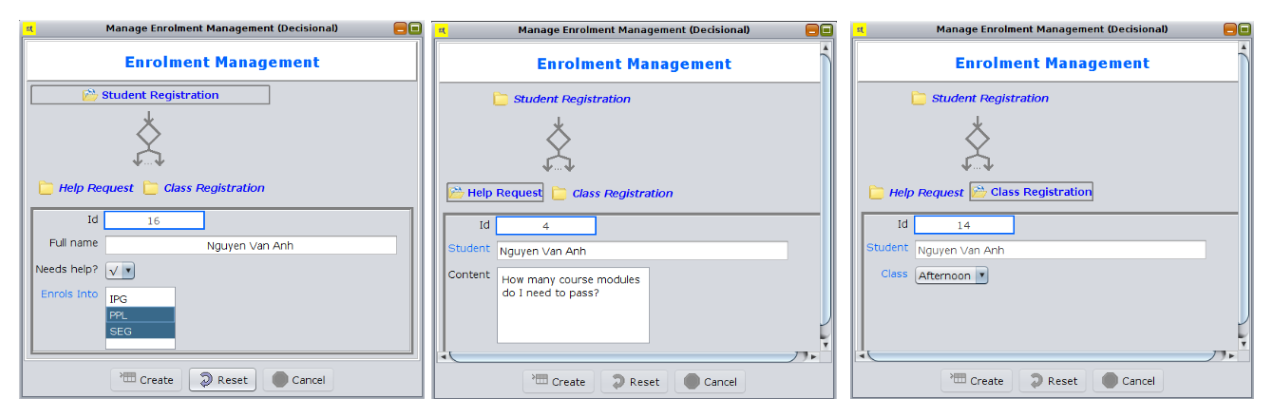
\includegraphics[scale=0.64]{decisional-form-eg-gui}
	\end{center}
	\vspace{-0.5cm}
	\caption{The decisional pattern form view of enrolment management.} %
	\label{fig:decisional-form-eg-gui}
	\vspace{-0.4cm}
\end{figure}

%\noindent Figure~\ref{fig:decisional-form-eg-gui} shows the three GUI snapshots of the example. The first GUI is for student registration. The second and third GUIs are for the cases that help request is and is not requested (\resp). The activity's GUI contains the GUIs of the three actions in separate tabs. Under both cases of the decision, the \clazz{Student} object that is created in the first action (\eg \clazz{Student}(\attribn{name}=``Nguyen Van Anh'')) is passed on to the next action. This object is then presented in the data field of the associative field \attribn{student} of the domain class referenced by this action.
Figure~\ref{fig:decisional-form-eg-gui} shows three snapshots of the GUI for this example. The first GUI is for student registration, while the second and third GUIs are for the cases where help request is and is not requested (\resp). The activity's GUI contains the GUIs of the three actions in separate tabs. In both cases of the decision, the \clazz{Student} object that is created in the first action (\eg \clazz{Student}(\attribn{name}=``Nguyen Van Anh'')) is passed on to the next action. This object is then displayed in the data field of the associative field \attribn{student} of the domain class referenced by this action.

%%%%%%%%%%%%%%%%%%%%%%%%%%%%%%%%%%%%%%%%%%%%%%%%%%%%%%% 
\subsection{Applying Domain Behavior Patterns}
%\label{subsect:applyBehaviorPatterns}
%%%%%%%%%%%%%%%%%%%%%%%%%%%%%%%%%%%%%%%%%%%%%%%%%%%%%%%

To obtain a concrete \agl~specification when applying a domain behavior pattern, basically, we follow three main steps:
\begin{enumerate}
	\item Representing the input UML Activity diagram and the template configured unified model of the pattern as activity graphs; 
	\item %Defining the matching of the template on the activity in order to define ANodes, their sequence, and domain classes referenced by them. The reference from ANodes to domain classes (expressed with the keywords \attribn{refCls} and \attribn{outCles}) provides a mapping between the activity and the unified class model;	
	Defining the matching of the template to the activity in order to define \clazz{ANode}s, their sequence, and the domain classes referenced by them. The reference from \clazz{ANode}s to domain classes (expressed with the keywords \attribn{refCls} and \attribn{outCls}) provides a mapping between the activity and the unified class model;
	\item %Defining the generic behavior (expressed by a SAA with the keyword \attribn{actSeq}) of the domain module \wrt the domain class referenced by each ANode. This helps synchronize the execution state of the activity and the current state of the unified class model.	
	Expressing the generic behavior of the domain module \wrt the domain class referenced by each ANode through a SAA using the keyword \attribn{actSeq}. This ensures that the execution state of the activity is synchronized with the current state of the unified class model.
\end{enumerate} 

% We would further explain this procedure and illustrate it with an example in Section~\ref{subsect:agl-abstractSyntax}. 

\begin{figure}[ht]
	\centering
	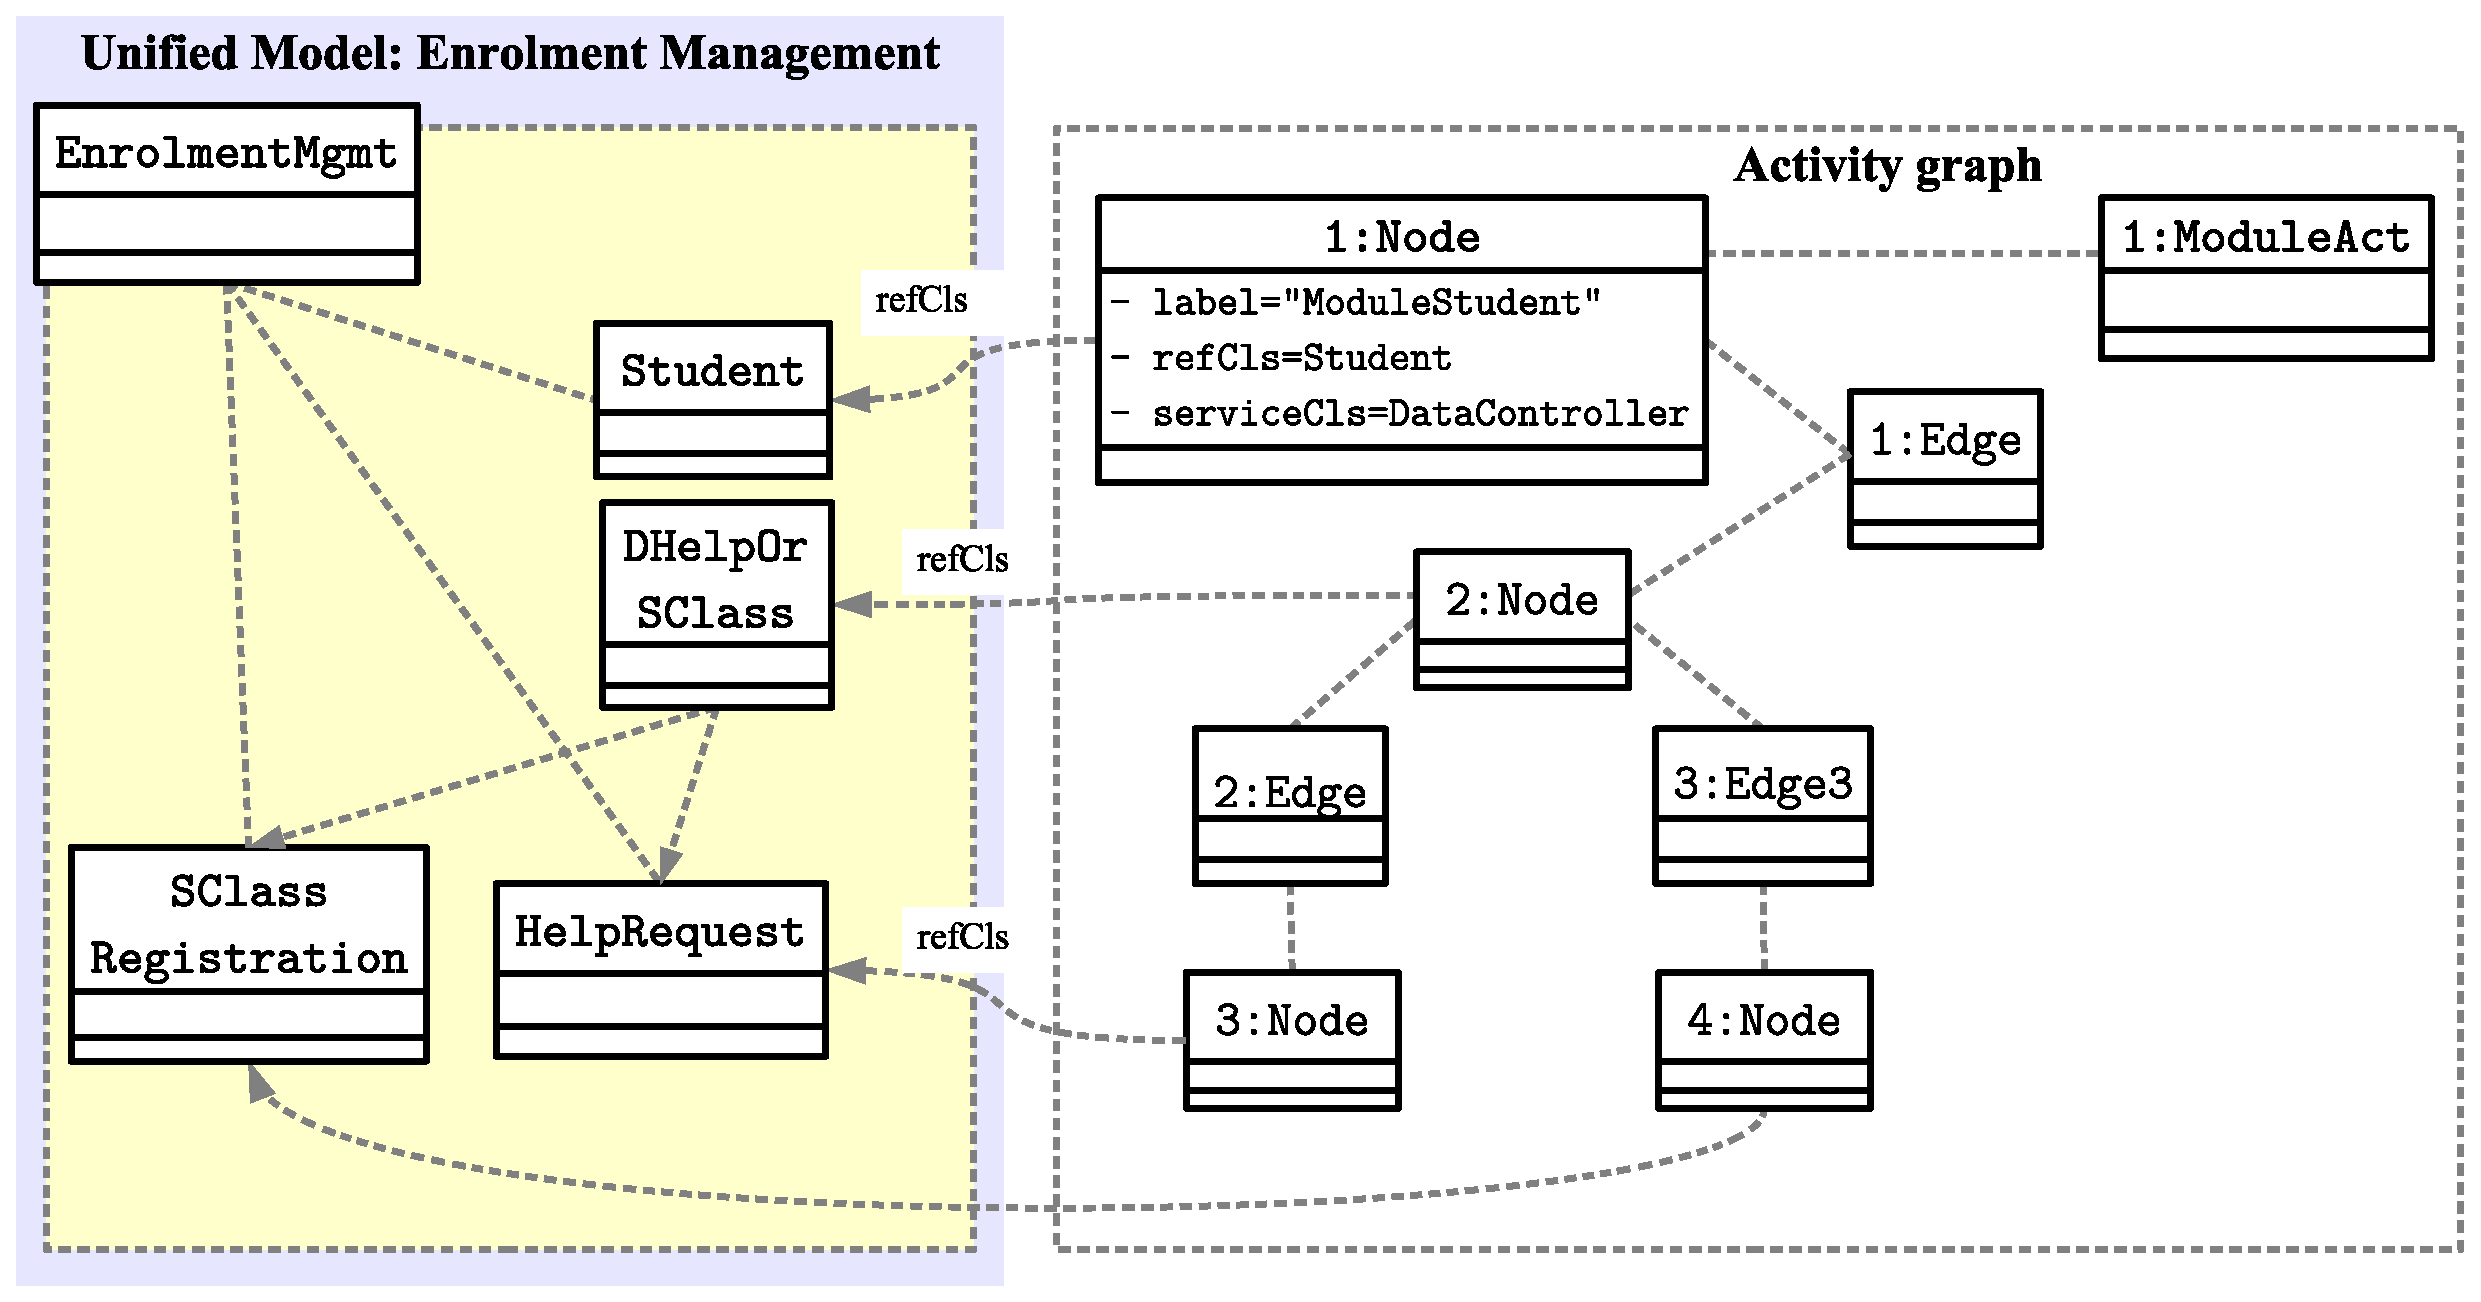
\includegraphics[scale=0.28]{activity-graph-example}
	\caption{(LHS) A repeat of the unified class model shown in Figure~\ref{fig:unified-model-example}; (RHS) The activity graph of this model.} %
	\label{fig:activity-graph-example}
\end{figure}

% TODO: + tab:activity-graph-example
% + add a separate table for ModuleAct objects and reference them in the actSeq column
\begin{table*}[ht]
	\setlength\tabcolsep{5pt}
	\begin{center} \footnotesize
		\caption{(A: Top) \clazz{Node} objects, (B: Bottom-left) \clazz{Edge} objects of the activity graph in Figure~\ref{fig:activity-graph-example} and (C: Bottom-right)  
			\clazz{ModuleAct} objects that are referenced by the \clazz{Node}s}\label{tab:activity-graph-example}
		%
		\begin{tabular}{|>{\centering\arraybackslash}m{0.7cm}|>{\centering\arraybackslash}m{3.5cm}|>{\centering\arraybackslash}m{3cm}|>{\centering\arraybackslash}m{2.5cm}|>{\centering\arraybackslash}m{5cm}|}
			%content
			\hline
			\rowcolor{lightgray}
			\textbf{Node-Id} & \textbf{\attribn{label}} & \textbf{\attribn{refCls}} & \textbf{\attribn{serviceCls}} & \textbf{\attribn{actSeq}} \\\hline
			1 & \strq{MStudent} & \clazz{Student} & \clazz{DataController} & [\objid{1}{ModuleAct}]\\\hline 
			2 & \strq{MDHelpOrSClass} & \clazz{DHelpOrSClass} & \code{null} & \code{null}\\\hline 
			3 & \strq{MHelpRequest} & \clazz{HelpRequest} & \clazz{DataController} & [\objid{2}{ModuleAct}, \objid{3}{ModuleAct}]\\\hline 
			4 & \strq{MSClassRegistration} & \clazz{SClassRegistration} & \clazz{DataController} & [\objid{4}{ModuleAct}, \objid{5}{ModuleAct}]\\\hline
		\end{tabular} 
		%
		\begin{tabular}{|>{\centering\arraybackslash}m{0.7cm}|>{\centering\arraybackslash}m{2cm}|>{\centering\arraybackslash}m{2cm}|}
			%content
			\hline
			\rowcolor{lightgray}
			\textbf{Edge-Id} & \textbf{\attribn{n1}} & \textbf{\attribn{n2}} \\\hline
			1 & \objid{1}{Node} & \objid{2}{Node} \\\hline 
			2 & \objid{2}{Node} & \objid{3}{Node} \\\hline 
			3 & \objid{2}{Node} & \objid{4}{Node} \\\hline 
		\end{tabular}
		%
		\begin{tabular}{|>{\centering\arraybackslash}m{1cm}|>{\centering\arraybackslash}m{3cm}|>{\centering\arraybackslash}m{2cm}|>{\centering\arraybackslash}m{2cm}|}
			%content
			\hline
			\rowcolor{lightgray}
			\textbf{MAct-Id} & \textbf{\attribn{actName}} & \textbf{\attribn{postStates}} & \textbf{\attribn{fieldNames}} \\\hline
			1 & \membern{newObject} & \set{Created} & \\\hline 
			2 & \membern{newObject} & \set{NewObject} & \\\hline 
			3 & \membern{setDataFieldValues} & \set{Created} & \sets{\strq{student}} \\\hline 
			4 & \membern{newObject} & \set{NewObject} & \\\hline 
			5 & \membern{setDataFieldValues} & \set{Created} & \sets{\strq{student}} \\\hline 
		\end{tabular}
	\vspace{-0.2cm}
\end{center}\end{table*}

\noindent\textbf{Example.} 
%The right-hand side of Figure~\ref{fig:activity-graph-example} is an activity graph of the enrollment management activity of the \courseman~software variant introduced earlier in Section~\ref{sect:background}. The left-hand side of the figure is the corresponding unified class model of this activity, which is repeated from Figure~\ref{fig:unified-model-example} to show links with the activity graph. 
Figure~\ref{fig:activity-graph-example} shows \courseman's enrollment management activity graph on the right-hand side, while the corresponding unified class model is shown on the left-hand side.
%We will discuss other example graphs that include control nodes later in Section~\ref{sect:eval-expressiveness}. 
%Other example graphs that include control notes are mentioned in SubSection~\ref{sect:incorporatePatterns}.
Tables~\ref{tab:activity-graph-example}(A) and (B) list the states of the nodes and edges (\resp) of the activity graph. Table~\ref{tab:activity-graph-example}(C) lists the \clazz{ModuleAct} objects that are referenced by the \clazz{Node}s in Table~\ref{tab:activity-graph-example}(A). A \clazz{ModuleAct} object represents an SAA. Each table column lists the values of a representative field of an object.
%
For instance, node \objid{1}{Node} references the domain class \clazz{Student} (hence also references \clazz{ModuleStudent}) and has \membern{serviceCls} = \clazz{DataController} (a default module service class developed as part of the \jdomainapp~framework~\cite{le_jdomainapp_2017}). The node also references object \objid{1}{ModuleAct}. The \membern{refCls} field of each node is depicted in the figure using a dashed curve labeled \strq{refCls} that connects the node to the referenced domain class.% in the unified class model.

We provide Definition~\ref{def:software} to clarify how the software is generated in MOSA. This definition makes precise the general notion of module-based software that we introduced in Section~\ref{sect:bg-arch} and takes into account the composition of a unified class model and an activity graph. It highlights the sub-set of modules that owns the activity classes and how these modules handle the execution of the associated activity graphs.

\begin{definition} \label{def:software}
	Given a unified class model that contains a non-empty set of activity classes, each of which is attached to an AGL specification describing the activity graph logic of a domain activity. \textit{A unified domain model} $D$ is a composition of the unified class model and the AGL specifications. A software generated in MOSA \wrt $D$ consists in a set of modules, each of which owns a domain class in $D$ and the behavior of the \code{newObject} action of every owner module of an activity class includes the logic described by the activity graph that is configured by the AGL specification attached to that class. \qed
\end{definition}

%
%%%%%%%%%%%%%%%%%%%%%%%%%%%%%%%%%%%%%%%%%%%%%%%%%
%\subsection{Forked Pattern Form} \label{sect:forked-pattern}
%%%%%%%%%%%%%%%%%%%%%%%%%%%%%%%%%%%%%%%%%%%%%%%%%
%
%The top-left of Figure~\ref{fig:forked-form} shows the UML activity model, while the top-right shows the template configured unified model. The activity class \clazz{Ca} has two associations to domain class \clazz{Cf} (referenced by node $ e_f $) and control class \clazz{Co} (referenced by the forked node). Class \clazz{Co} in turn has associations to the other three domain classes, namely \clazz{C1}, \clazz{Cn}, and \clazz{Ck}. In addition to these, class \clazz{Cf} has two associations to \clazz{C1} and \clazz{Cn}, as these classes need to know \clazz{Cf} through object passing.
%%
%Similar to the decisional activity's template model, we consider the case that the class \clazz{Ck} is not a decision class. When this class is a decision class, we unfold it into the template model.
%%
%The AGC is very similar to that of the decisional activity's template model, except for in the second \clazz{ANode}: the reference class is \clazz{Co} (as opposed to \clazz{D}), the node type is \code{Fork} and property \attribn{serviceCls} is \clazz{DataController}. This property configuration makes explicit the fact that \clazz{Co}'s module service is available for use if needed.
%
%\begin{figure}%[ht]
%	\begin{center}
%		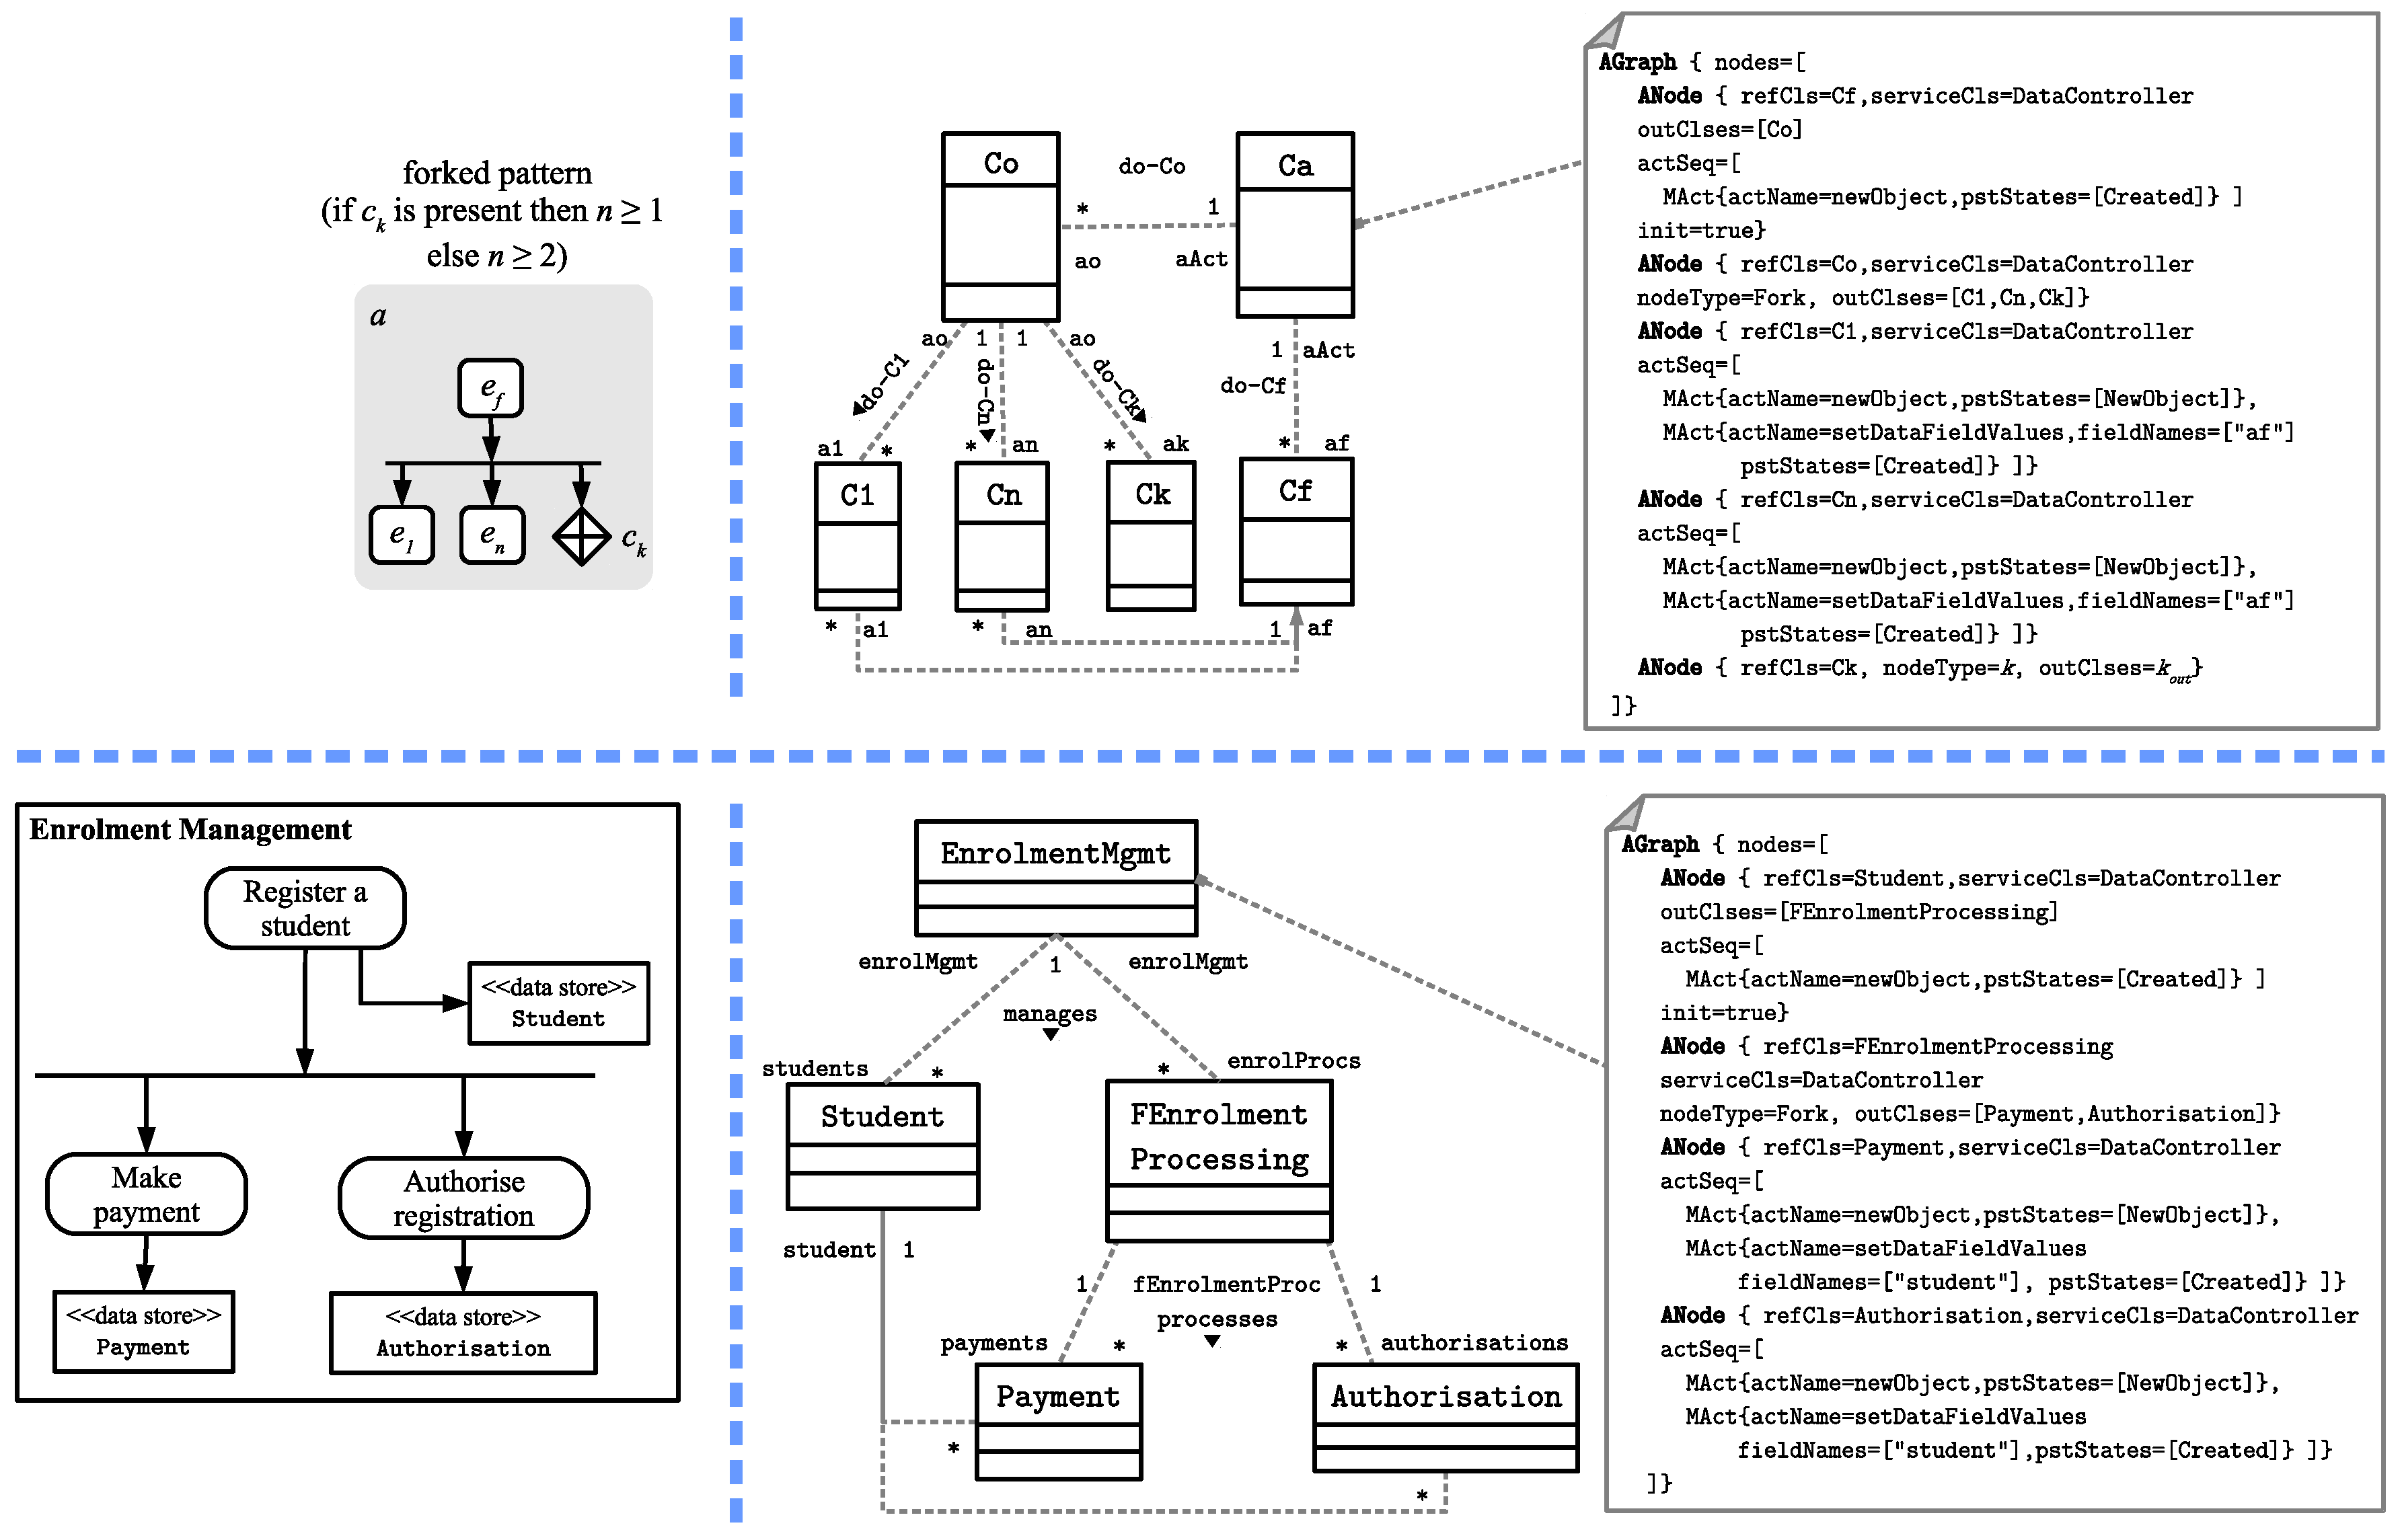
\includegraphics[scale=0.27 % 0.3
%		]{case-study/forked-form}
%	\end{center}
%	\caption{The forked pattern form.} %
%	\label{fig:forked-form}
%\end{figure}
%
%\begin{figure}
%	\begin{center}
%		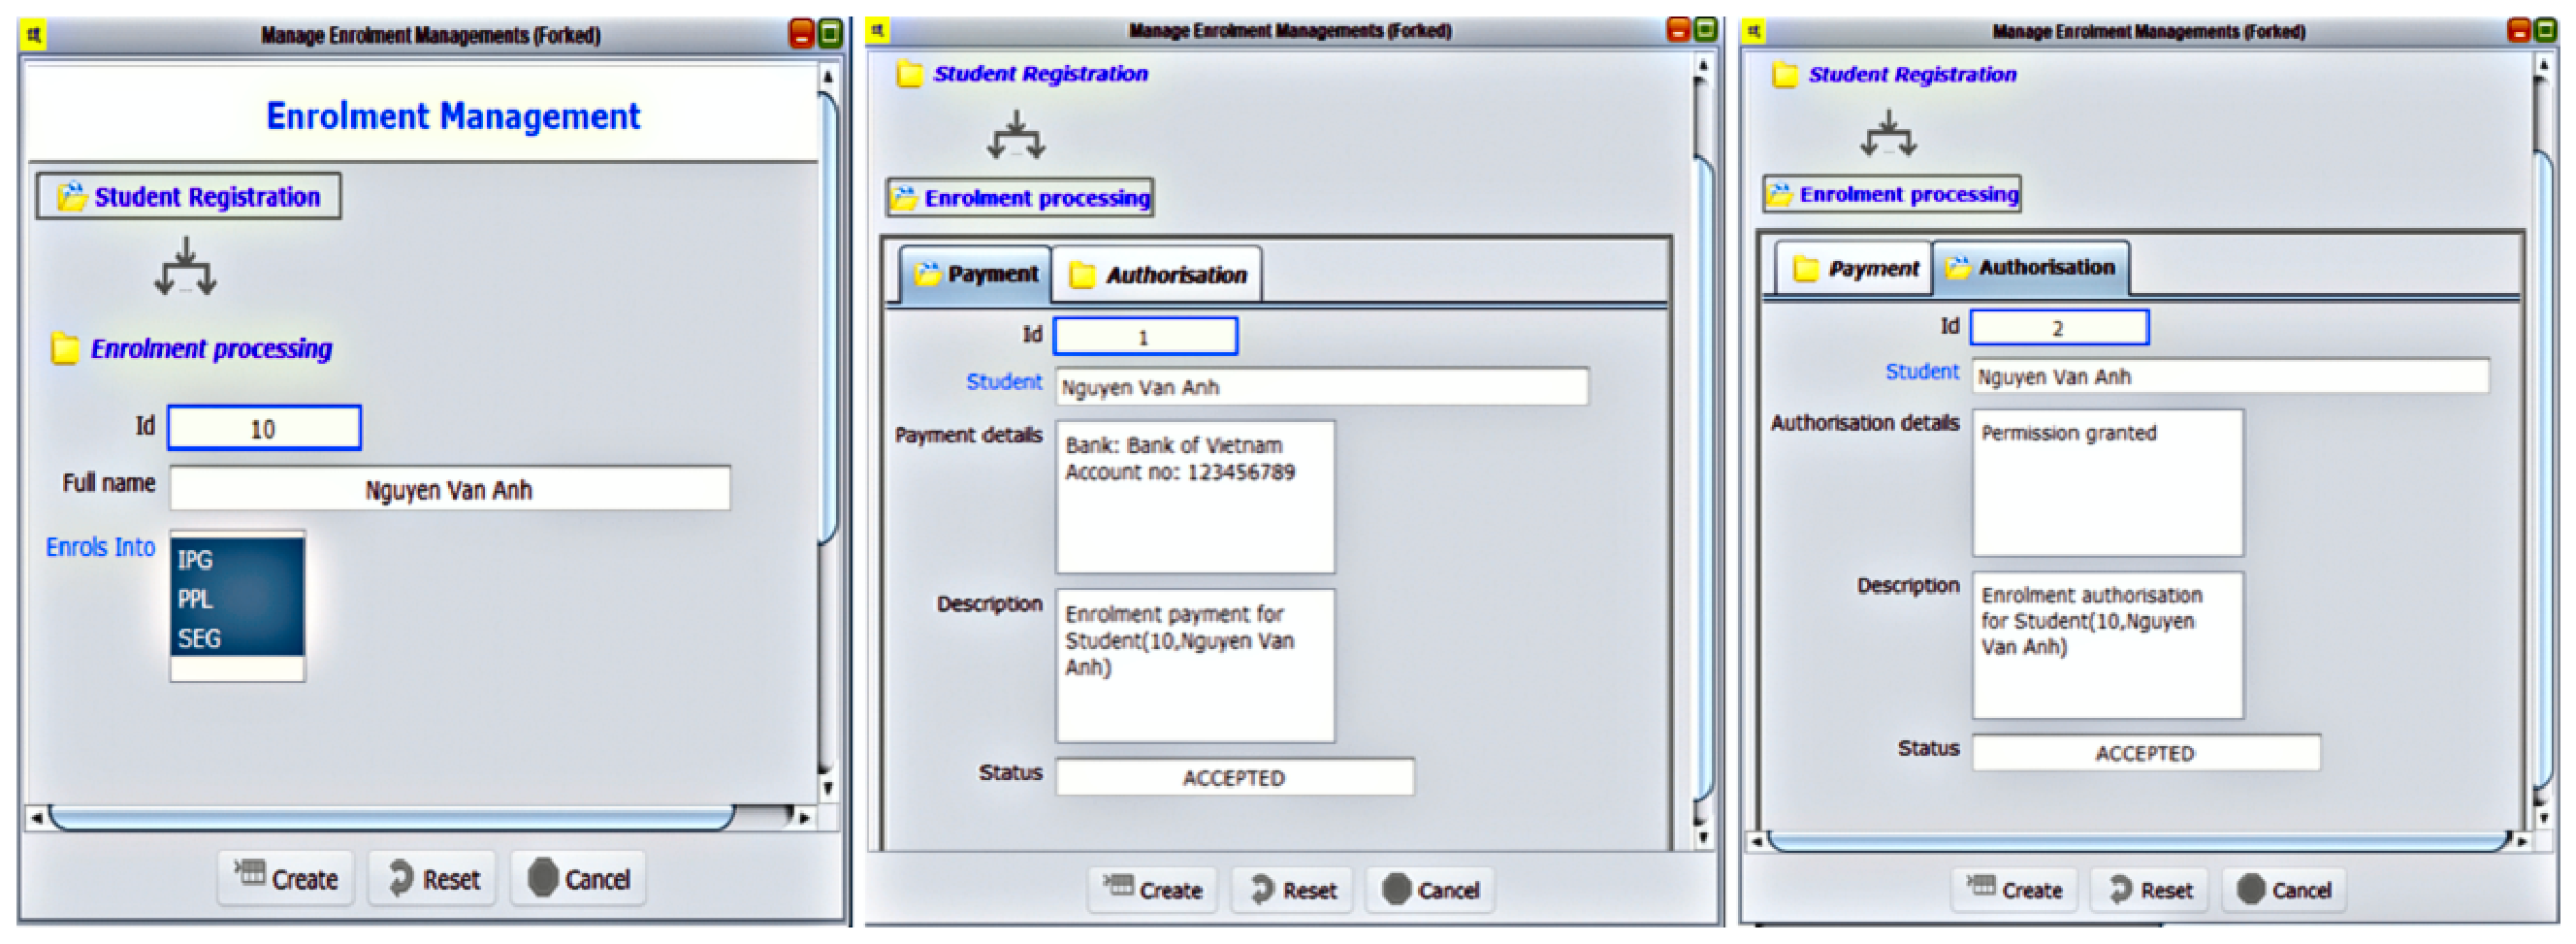
\includegraphics[scale=0.36 %0.4
%		]{case-study/forked-form-eg-gui}
%	\end{center}
%	\caption{The forked pattern form view of enrolment management activity.} %
%	\label{fig:forked-form-eg-gui}
%\end{figure}
%
%\subsubsection*{Example}
%The bottom of Figure~\ref{fig:forked-form} shows how the pattern is applied to another variant of the \courseman's enrolment management. The UML activity model of this variant involves performing student registration ($ e_f $) and then two support actions concurrently: payment processing ($ e_1 $) and enrolment authorisation ($ e_2 $). These actions must be completed in order for any subsequent actions to proceed.
%%
%In this example: \clazz{Ca} = \clazz{EnrolmentMgmt}, \clazz{Cf} = \clazz{Student}, \clazz{Co} = \clazz{FEnrolmentProcessing}, $ n = 2 $, \clazz{C1} = \clazz{Payment}, \clazz{C2} = \clazz{Auhorisation}.
%
%The three GUI snapshots of the example are shown in Figure~\ref{fig:forked-form-eg-gui}: one snapshot for one action. The first snapshot is for the first action \textit{student registration}. The second and third snapshots are for the two concurrent actions (\resp): \textit{making payment} and \textit{enrolment authorisation}. A difference between this pattern and the the previous two patterns is that this GUI has a 2-level containment. This 2-level containment reflects the length-2 association chain from \clazz{EnrolmentMgmt} (the activity class) to \clazz{Payment} and \clazz{Authorisation}. The first-level containment connects the activity's GUI with \clazz{Student}'s and enrolment processing's GUI. The second-level containment connects enrolment processing's GUI with \clazz{Payment}'s and \clazz{Authorisation}'s GUI.
%
%%%%%%%%%%%%%%%%%%%%%%%%%%%%%%%%%%%%%%%%%%%%%%%%%
%\subsection{Joined Pattern Form} \label{sect:joined-pattern}
%%%%%%%%%%%%%%%%%%%%%%%%%%%%%%%%%%%%%%%%%%%%%%%%%
%
%The top-left of Figure~\ref{fig:joined-form} shows the UML activity model, while the top-right shows the template configured unified model. The activity class \clazz{Ca} has associations to the domain classes \clazz{C1}, \clazz{Cn}, \clazz{Ck}, and \clazz{Cj}. These classes are referenced by the activity nodes $ e_1 $, $ e_n $, $ c_k $, and $ e_j $ (\resp). Class \clazz{Cj} has two associations to \clazz{C1} and \clazz{Cn}, as it knows these two classes through object passing. Class \clazz{J} implements the interface \clazz{Join} for the join logic.
%
%\begin{figure*}[ht]
%\begin{center}
%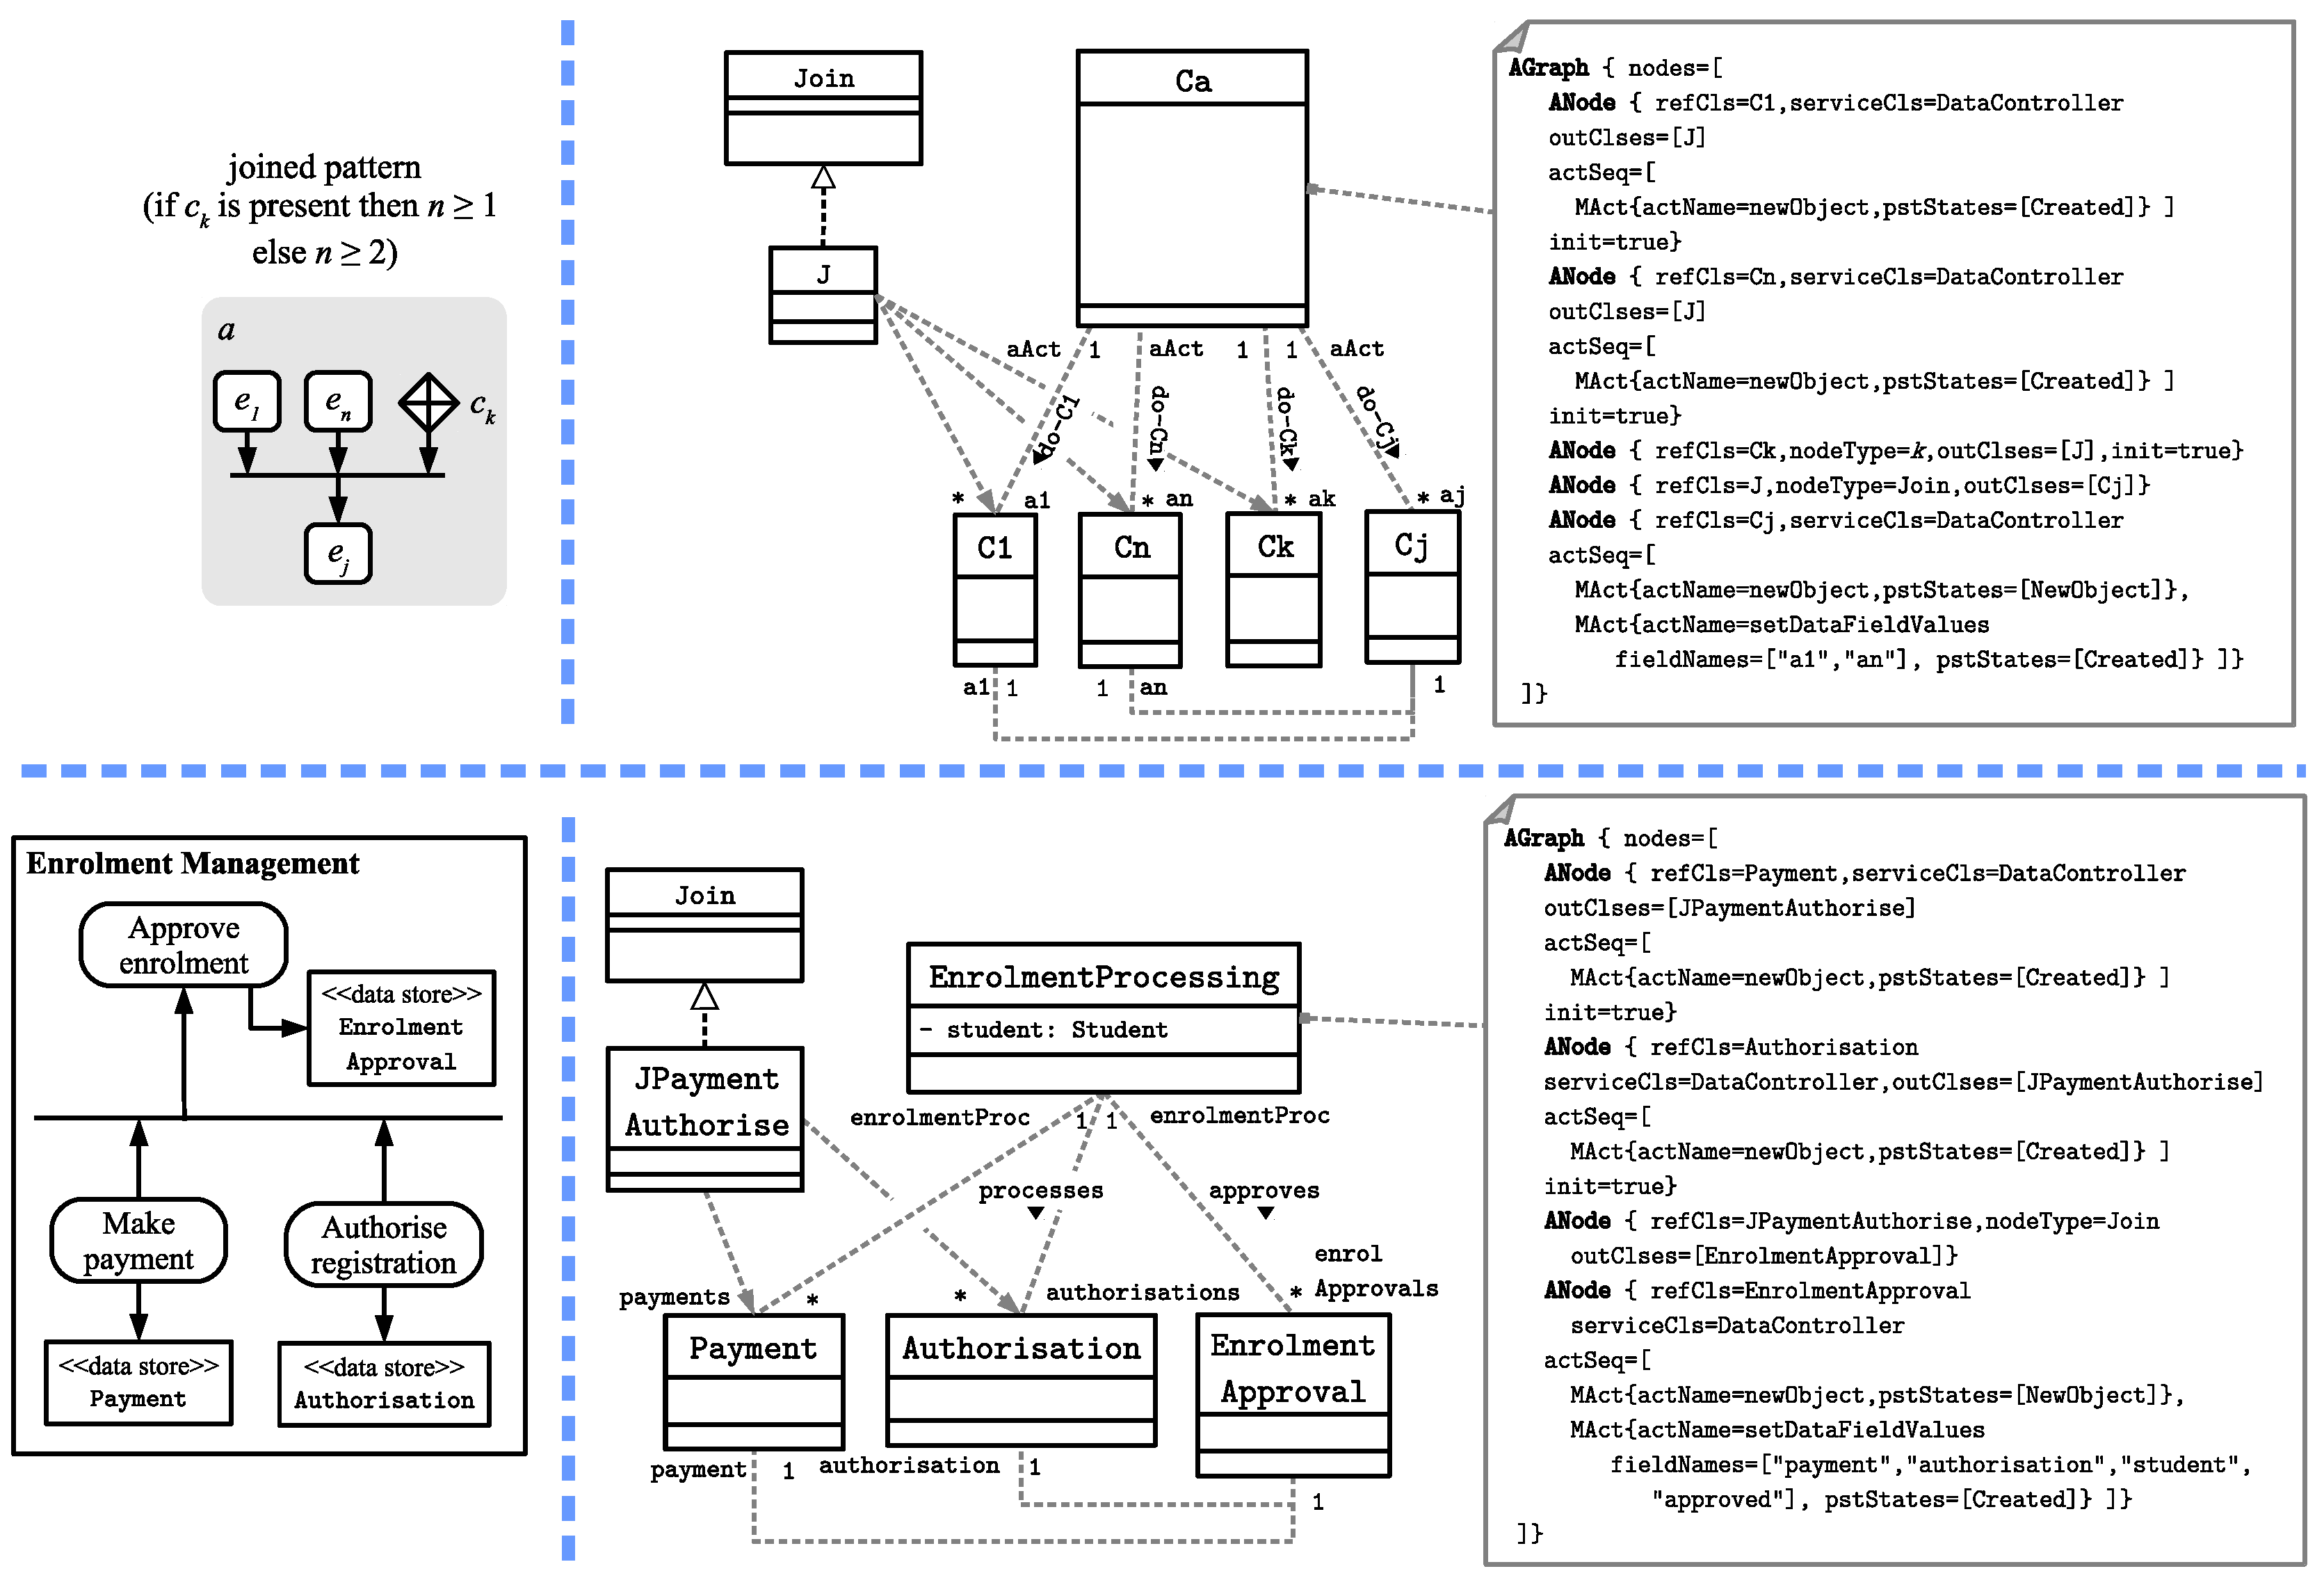
\includegraphics[scale=0.30 %0.3
%  ]{case-study/joined-form}
%\end{center}
%\caption{The joined pattern form.} %
%\label{fig:joined-form}
%\end{figure*}
%
%Similar to the decisional activity's template model, we create three (optional) weak dependency associations between class \clazz{J} and three domain classes \clazz{C1}, \clazz{Cn}, and \clazz{Ck}. In addition, we consider the case that the class \clazz{Ck} is not a decision class. When this class is a decision class, we unfold it into the template model.
%
%The AGC consists of five \clazz{ANode}s. The first three \clazz{ANode}s configure the three start nodes $ e_1 $, $ e_n $, and $ c_k $; and thus they all have \attribn{init}=\code{true} and \attribn{outClses} pointing to the domain class \clazz{J}. This class, which realises the interface \clazz{Join}, is referenced by the fourth \clazz{ANode}. This \clazz{ANode} configures the join node, and thus has \attribn{nodeType}=\clazz{Join}. The last \clazz{ANode} configures the last node $ e_j $. It specifies two \clazz{MAct}s, the second of which references the action  \membern{setDataFieldValues} which sets the view field values of the two fields \strq{a1} and \strq{an}. The input for this operation is the output of the operation \clazz{Join}.\membern{transf}.
%%
%\subsubsection*{Example}
%The bottom of Figure~\ref{fig:joined-form} shows how the pattern is applied to another variant of the \courseman's enrolment management activity. The UML activity model of this variant involves joining two actions that concern the same \clazz{Student}, namely making payment ($e_1$) and registration authorisation ($e_2$), before concluding at the enrolment approval action. This last action decides, based on the results of the other two actions, whether or not to approve the student enrolment.
%
%In this example: \clazz{Ca} = \clazz{EnrolmentMgmt}, $ n = 2 $, \clazz{C1} = \clazz{Payment}, \clazz{C2} = \clazz{Auhorisation}, \clazz{J} = \clazz{JPaymentAuthorise}, \clazz{Cj} = \clazz{EnrolmentApproval}.
%Note that in addition to the newly added associations in the example model, class \clazz{EnrolmentProcessing} is added with a domain field \attribn{student}, which is used to obtain input from the user for a \clazz{Student}. This \clazz{Student} object is needed to initialise the payment and authorisation processes.
%
%\begin{figure*}[ht]
%	\begin{center}
%		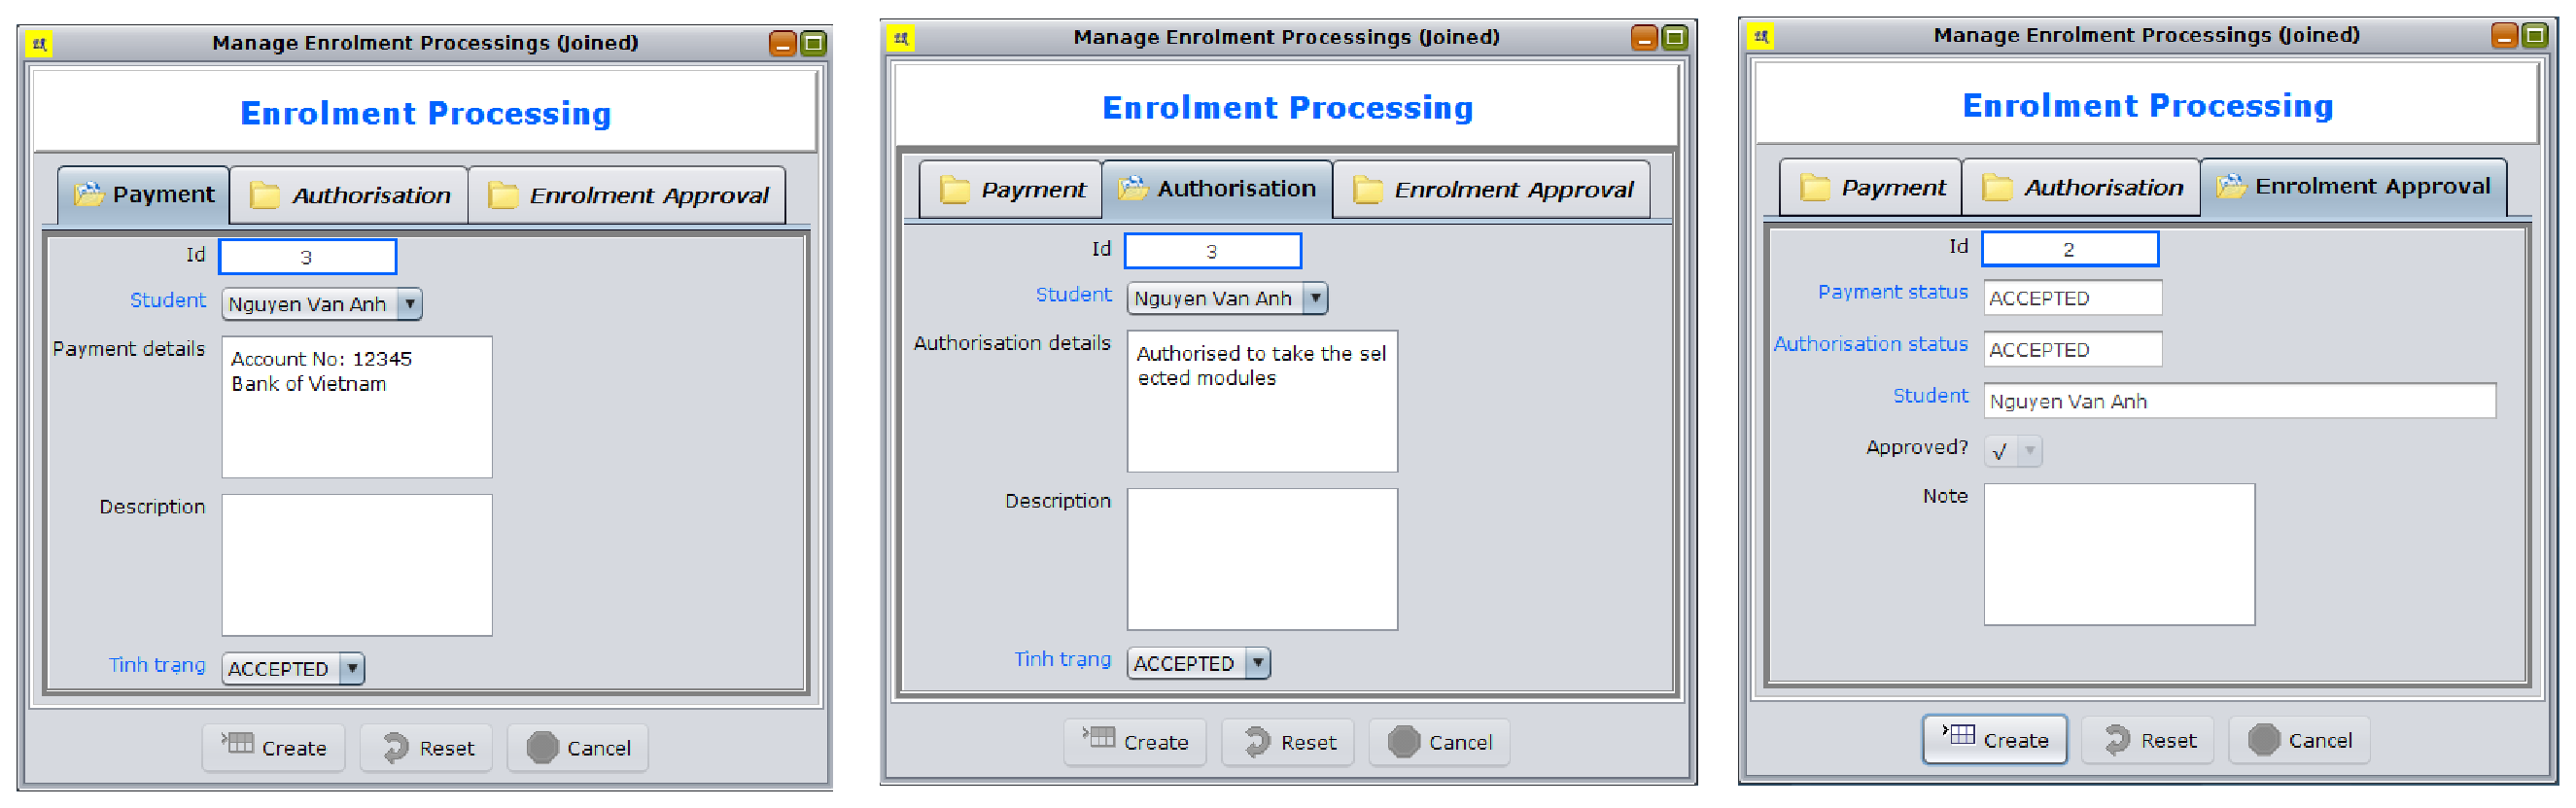
\includegraphics[scale=0.38 %0.4
%		]{case-study/joined-form-eg-gui}
%	\end{center}
%	\caption{The joined pattern form view of enrolment management activity.} %
%	\label{fig:joined-form-eg-gui}
%\end{figure*}
%
%The three GUI snapshots of the example are shown in Figure~\ref{fig:joined-form-eg-gui}: the first snapshot is for making payment, the second is for registration authorisation, and the third is for enrolment approval.
%
%%%%%%%%%%%%%%%%%%%%%%%%%%%%%%%%%%%%%%%%%%%%%%%%%
%\subsection{Merged Pattern Form} \label{sect:merged-pattern}
%%%%%%%%%%%%%%%%%%%%%%%%%%%%%%%%%%%%%%%%%%%%%%%%%
%
%The top-left of Figure~\ref{fig:merged-form} shows the UML activity model, while the top-right shows the template configured unified model. The activity class \clazz{Ca} has associations to the domain classes \clazz{Cg} and \clazz{Cm}. These classes are referenced by the merge node and the activity node $ e_m $ (\resp). Class \clazz{Cg} has associations to the domain classes of the other nodes, namely \clazz{C1}, \clazz{Cn}, and \clazz{Ck}. Class \clazz{Cm} has associations to class \clazz{C1} and \clazz{Cn} as it knows these two classes through object passing.
%%
%Similar to the decisional activity's template model, we consider the case that class \clazz{Ck} is not a decision class. When this class is a decision class, we unfold it into the template model.
%%
%The AGC is very similar to that of the join pattern form, except for the configuration of the fourth \clazz{ANode}, which specifies that the node type be \clazz{Merge} rather than \clazz{Join}.
%
%\begin{figure*}%[ht]
%	\begin{center}
%		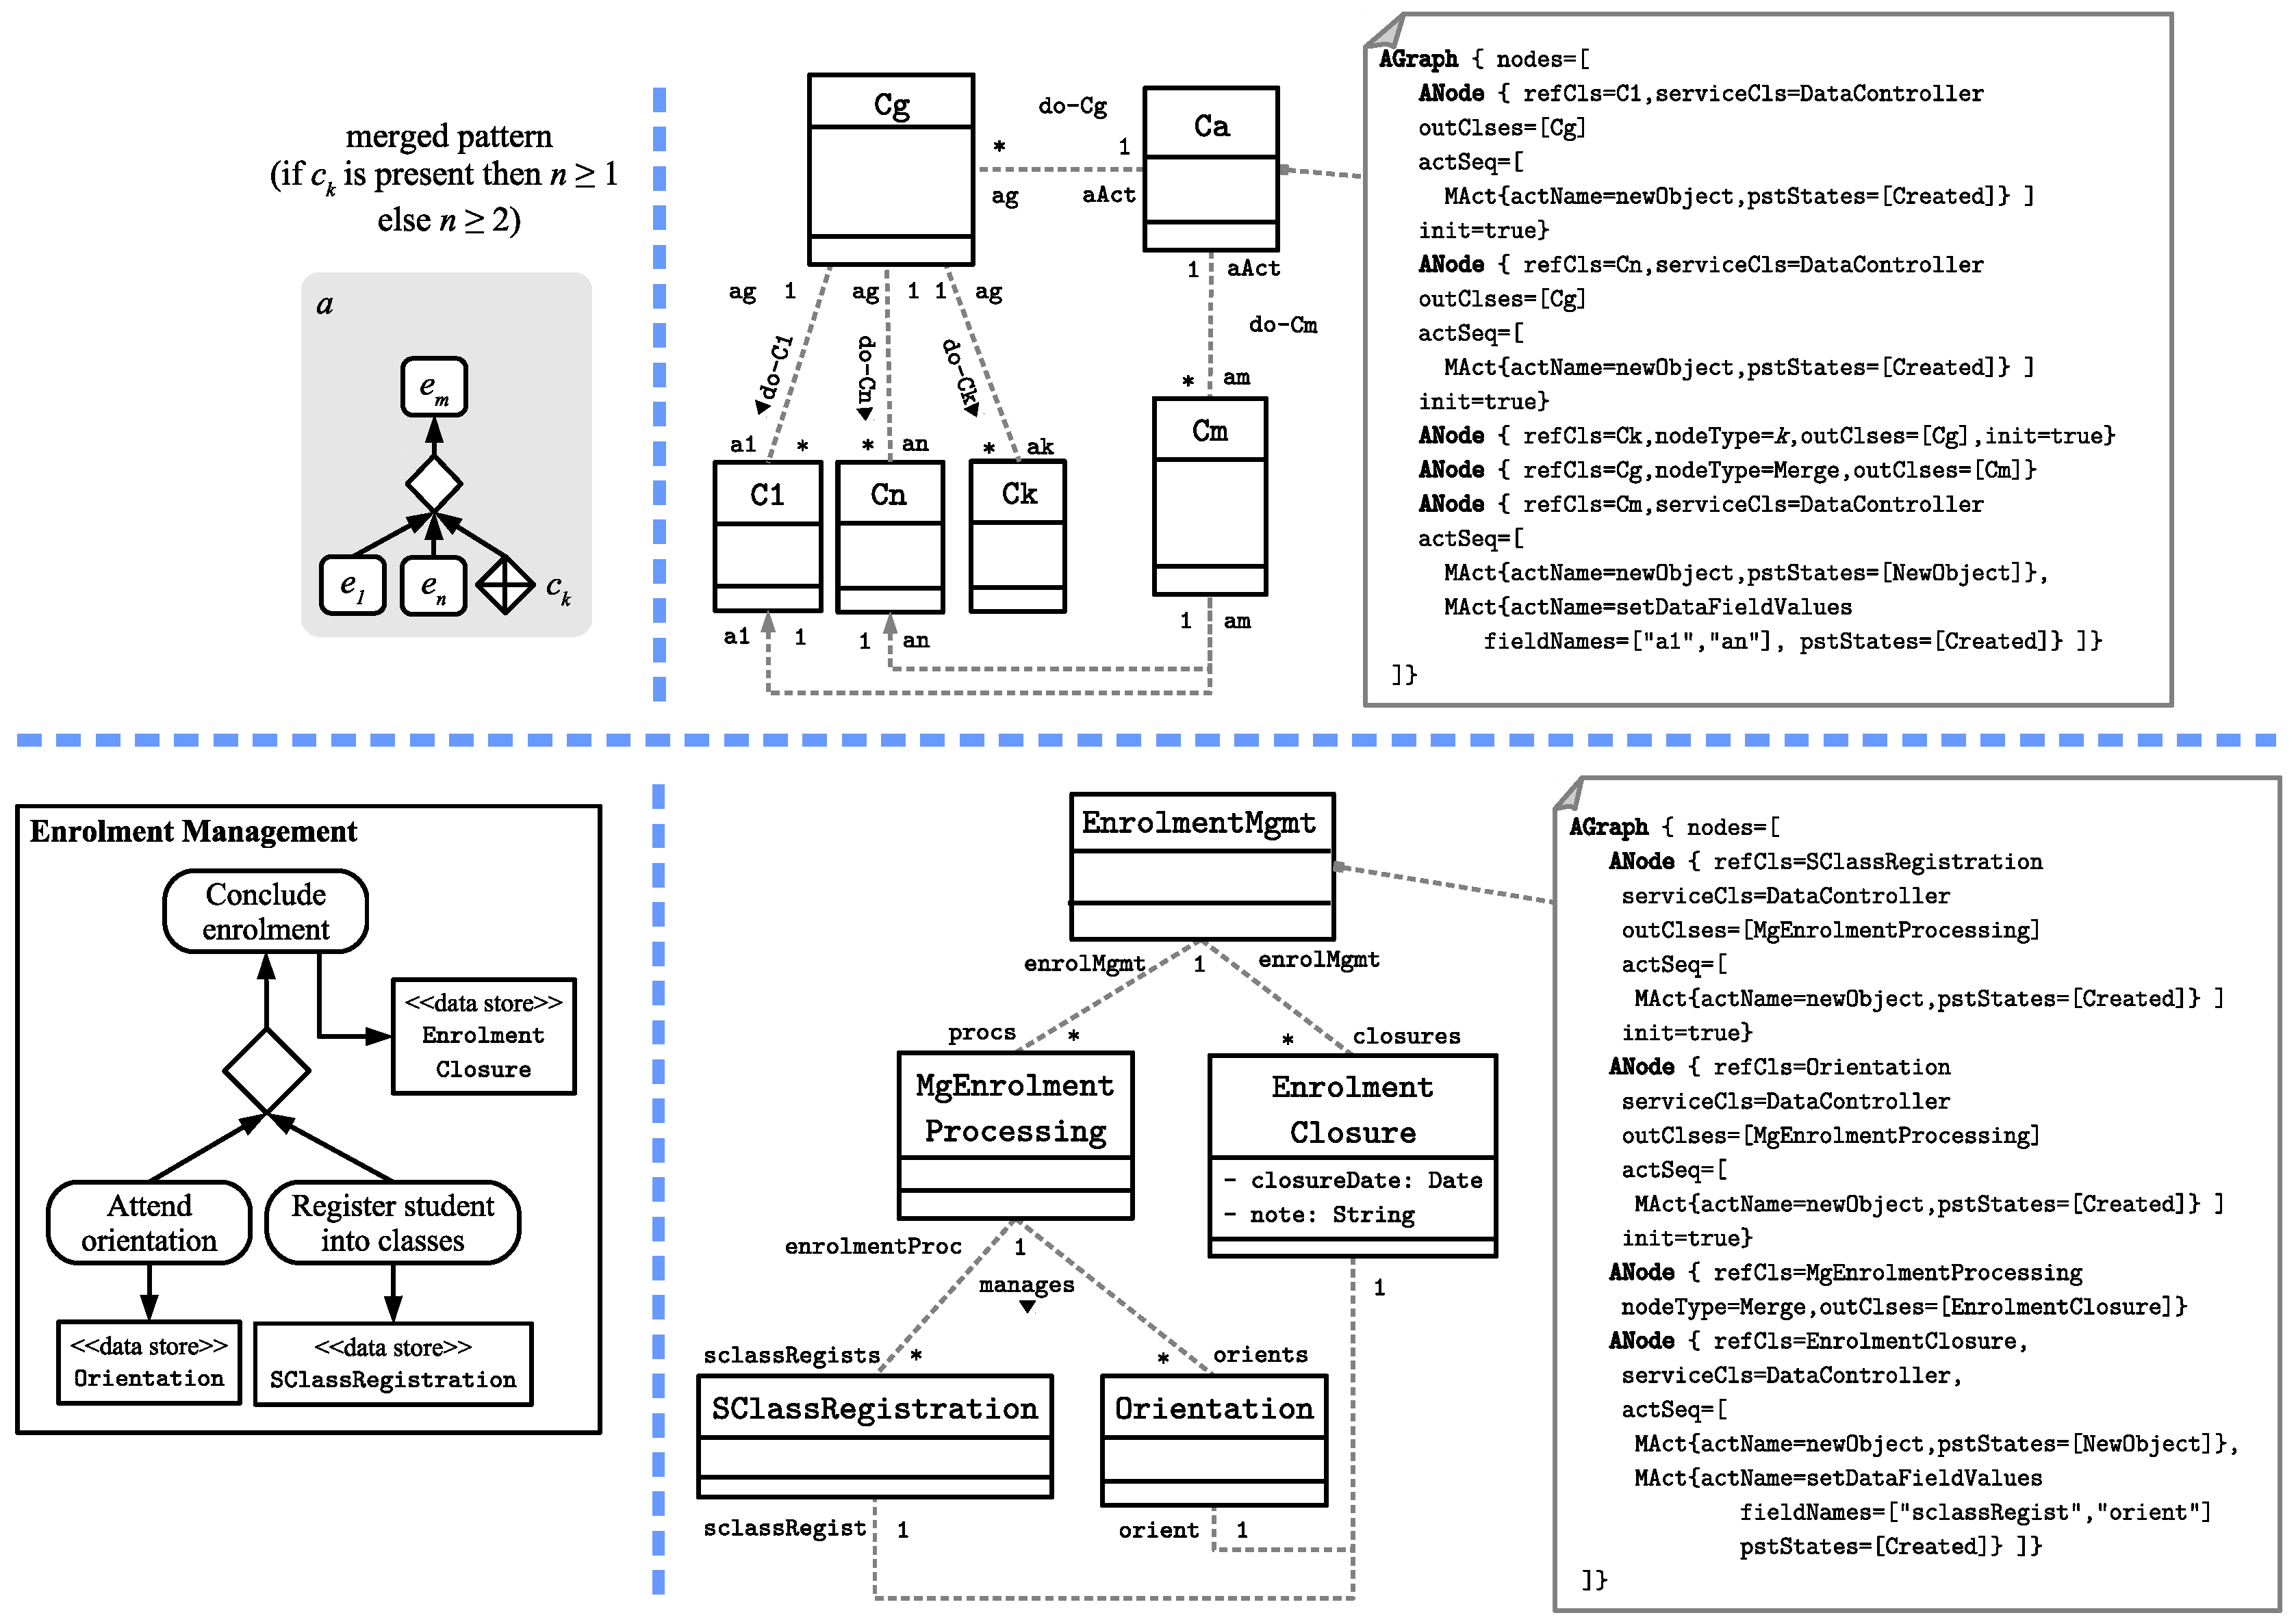
\includegraphics[scale=0.30 %0.3
%		]{case-study/merged-form}
%	\end{center}
%	\caption{The merged pattern form.} %
%	\label{fig:merged-form}
%\end{figure*}
%
%\begin{figure}%[ht]
%	\begin{center}
%		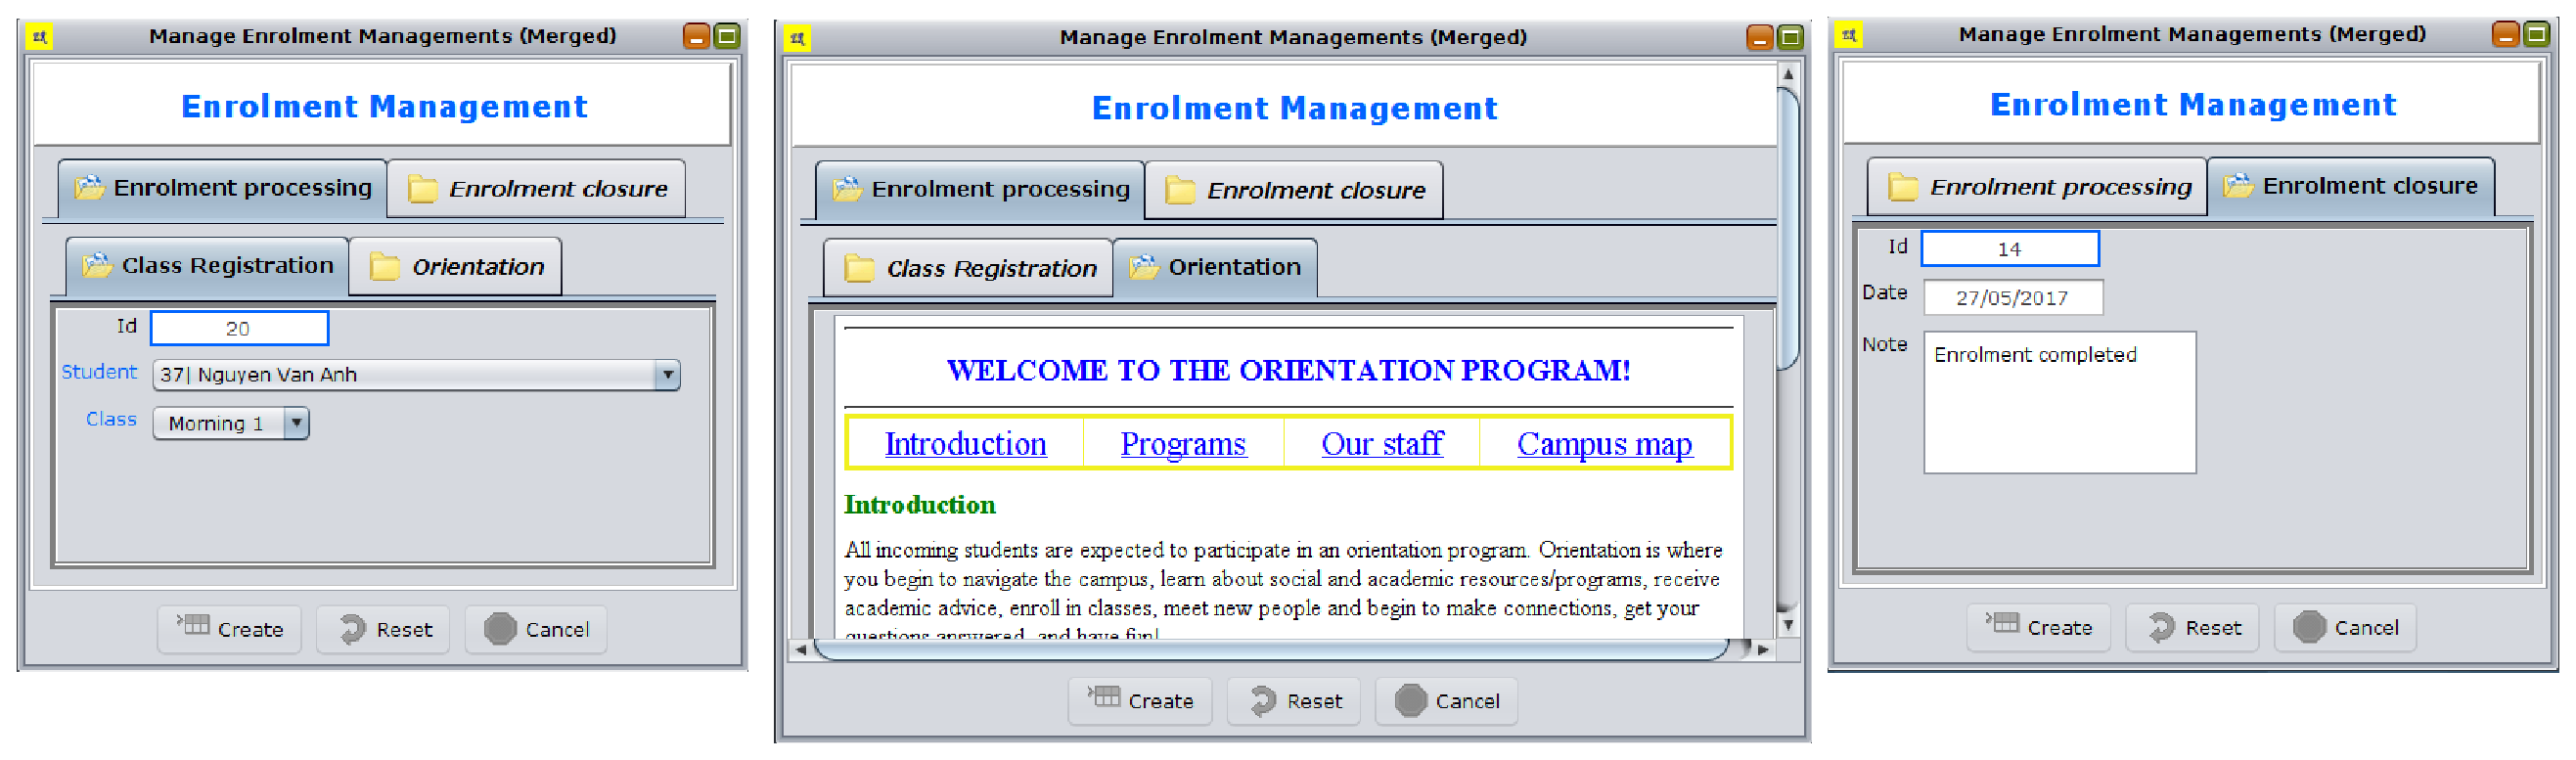
\includegraphics[scale=0.38 %0.4
%		]{case-study/merged-form-eg-gui}
%	\end{center}
%	\caption{The merged pattern form view of enrolment management activity.} %
%	\label{fig:merged-form-eg-gui}
%\end{figure}
%
%\subsubsection*{Example}
%The bottom of Figure~\ref{fig:merged-form} shows how the pattern is applied to another variant of the \courseman's enrolment management activity. The UML activity model of this variant involves merging two actions, namely student class registration ($e_1$) and attending an orientation ($e_2$), to conclude at the action enrolment closure ($e_m$). The assumption here is that students can perform any combination of the two actions $e_1, e_2$. The completion of any one action will lead to enrolment closure. The action that has not yet been performed can be performed by the students at some later time.
%
%Action $e_2$ requires adding a new domain class named \clazz{Orientation} to the \Name{CourseMan}'s domain model. This class is displayed at the bottom right of Figure~\ref{fig:merged-form}. Thus, in this example: \clazz{Ca} = \clazz{EnrolmentMgmt}, $ n = 2 $, \clazz{C1} = \clazz{SClassRegistration}, \clazz{C2} = \clazz{Orientation}, \clazz{Cg} = \clazz{MgEnrolmentProcessing}, \clazz{Cm} = \clazz{EnrolmentClosure}. 
%
%The GUI snapshots of the example are shown in Figure~\ref{fig:merged-form-eg-gui}. It shows a length-2 association chain from \clazz{EnrolmentMgmt} to \clazz{SClassRegistration} and \clazz{Orientation}. 
%%The first-level containment is that between the \clazz{EnrolmentMgmt}'s GUI and \clazz{MgEnrolmentProcessing}'s and \clazz{EnrolmentClosure}'s GUI. The second-level containment is that between \clazz{MgEnrolmentProcessing}'s GUI and \clazz{SClassRegistration}'s and \clazz{Orientation}'s GUI (the first and second snapshots). 
%The first-level containment connects the \clazz{EnrolmentMgmt}'s GUI with \clazz{MgEnrolmentProcessing}'s and \clazz{EnrolmentClosure}'s GUI. The second-level containment connects the \clazz{MgEnrolmentProcessing}'s GUI and \clazz{SClassRegistration}'s and \clazz{Orientation}'s GUI (the first and second snapshots). The \clazz{EnrolmentClosure}'s GUI is the third snapshot.
